\subsection{Povoamento da Base de Dados}

De forma a testar e demonstrar a carga suportada pela aplicação, é necessário a automatização do povoamento da base de dados. Assim, desenvolveu-se um \textit{script}, em \texttt{Python}, parametrizado com as quantidades e probabilidades dos tipos de dados a inserir. O \textit{output} deste \textit{script} é um ficheiro com um conjunto de \textit{queries} SQL, que efetuam o povoamento da base de dados. Assim, é possível indicar, por exemplo, a quantidade de utilizadores comuns, \texttt{InternalAccount}, que se pretende inserir na base de dados, bem como a probabilidade de determinado utilizador ser de um género específico (\textit{female}, \textit{male} e \textit{undefined}).


\subsection{Testes de Carga}

Após o povoamento da base de dados, prosseguiu-se para a realização de testes de carga, de forma a avaliar o desempenho da aplicação desenvolvida. O objetivo é perceber quantos utilizadores simultâneos a aplicação suporta, com um tempo de resposta aceitável.

\subsubsection{Ferramenta utilizada}
\label{sec:ferramenta_utilizada}

Para a realização dos testes de carga referidos, analisou-se um vasto leque de ferramentas que permitem efetuar os mesmos. Verificou-se a disponibilidade de dois tipos principais de \textit{software} capazes de realizar estes testes:

\begin{enumerate}
    \item Realiza a gravação da interação do utilizador com a interface, permitindo a utilização de \textit{think times} mais realistas.
    \item Efetua o envio de pedidos HTTP ao servidor aplicacional, havendo necessidade de especificar o tipo e estrutura dos mesmos.
\end{enumerate}

As ferramentas que se sobressaíram, relativamente ao primeiro tipo de \textit{software}, foram o \texttt{WebLoad} e o \texttt{NeoLoad}. Já para o segundo, destacou-se o \texttt{Apache JMeter} e o \texttt{Predator}. Entre estas ferramentas, optou-se pelo \texttt{Apache JMeter} pelo motivos indicados de seguida:

\begin{itemize}
    \item \texttt{WebLoad}: Não suporta a gravação das interações do utilizador com a interface, quando esta utiliza o \texttt{Vue.js};
    \item \texttt{NeoLoad}: Não suporta, por defeito, a utilização de API's externas, como por exemplo a do \textit{Google Maps}. Além disso, o objetivo não é captar a interação do utilizador com a interface, mas sim testar o limite do servidor aplicacional em termos de carga.
    \item \texttt{Predator}: Dificuldade de instalação da ferramenta no sistema operativo \texttt{Windows}.
\end{itemize}

Relativamente ao \texttt{Apache JMeter}, com o auxílio de breves tutoriais, conseguiu-se parametrizar todos os pedidos pretendidos com relativa facilidade. Para além disso, verificou-se que esta ferramenta permite a geração de todas as estatísticas necessárias para avaliar a performance da aplicação, tal como:

\begin{itemize}
    \item \texttt{View Results Tree}: Permite visualizar se os pedidos realizados foram respondidos correta ou incorretamente, bem como o conteúdo dos pedidos e respostas HTTP (teste de correção);
    \item \texttt{Graph Results}: Permite ter um visão geral do débito e tempo de resposta dos vários pedidos ao longo do tempo;
    \item \texttt{Response Times Over Time}: Permite visualizar o tempo de resposta dos pedidos ao longo do tempo;
    \item \texttt{Active Threads Over Time}: Permite visualizar as \textit{threads} ativas ao longo do tempo;
\end{itemize}

Adicionalmente, esta ferramenta permite realizar vários tipos de teste de performance. Para isso é necessário especificar os parâmetros apresentados na figura \ref{fig:jmeter_parametros}, sendo os que apresentam maior relevância para este projeto explicitados de seguida:

\begin{itemize}
    \item \textit{Number of Threads}: Representa o número total de utilizadores virtuais que executam o \textit{script} de teste;
    \item \textit{Ramp-up Period}: Indica quanto tempo demorará para alcançar o número de \textit{threads} definidas;
    \item \textit{Loop Count}: Indica o número de execuções do \textit{script} de teste, por cada utilizador virtual. Se o \textit{loop count} estiver marcado como \textit{forever}, novas \textit{threads} irão começar até que os testes sejam parados; 
    \item \textit{Scheduler - Duration}: Limita o intervalo de tempo no qual os \textit{scripts} de testes podem ser iniciados.
\end{itemize}

A partir deste parâmetros é possível definir dois tipos de testes úteis para o cumprimento do objetivo estabelecido inicialmente:

\begin{itemize}
    \item \texttt{Teste 1}: o número de \textit{threads} estabelecido executa tantas vezes como o valor de definido no \textit{loop count} o \textit{script} de teste, sendo estas execuções distribuídas pelo período de \textit{ramp-up}. Os parâmetros utilizados para este tipo de teste são destacados na figura \ref{fig:jmeter_parametros} a roxo e amarelo.
    \item \texttt{Teste 2}: o número de \textit{threads} estabelecido representa o valor máximo de utilizadores virtuais que estão a efetuar pedidos em simultâneo. Assim, no início do teste, este número de utilizadores vai crescendo linearmente até ao período de \textit{ramp-up}, momento a partir do qual se mantém constante (no máximo). A duração total do teste é definida pela duração do \textit{scheduler}. Os parâmetros utilizados para este tipo de teste são destacados na figura \ref{fig:jmeter_parametros} a roxo e verde. A quantidade de \textit{threads} ativas em cada instante, de acordo com este tipo de teste, é representada no gráfico apresentado na figura \ref{fig:jmeter_ramp_up_test}.
\end{itemize}

\begin{figure}[H]
    \centering
    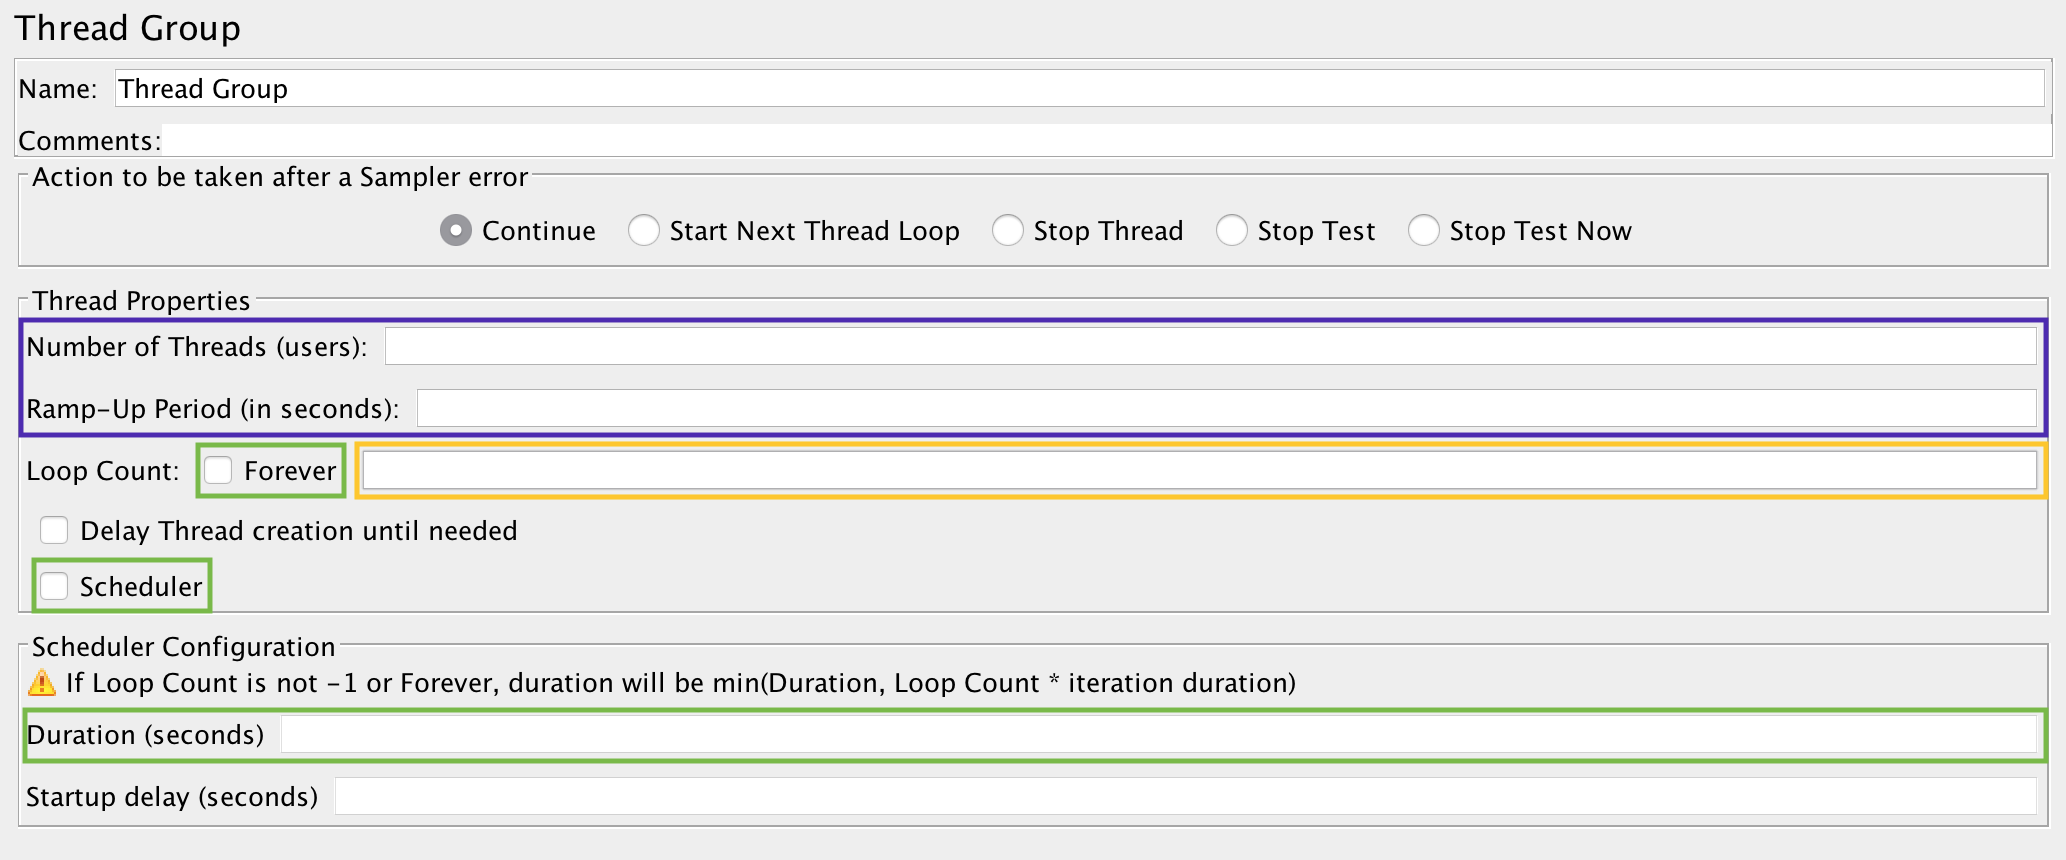
\includegraphics[width=1\textwidth]{images/Testes/ParametrosGroupThread.png}
    \caption{Parâmetros utilizados nos dois tipos de testes.}
    \label{fig:jmeter_parametros}
\end{figure}

\begin{figure}[H]
    \centering
    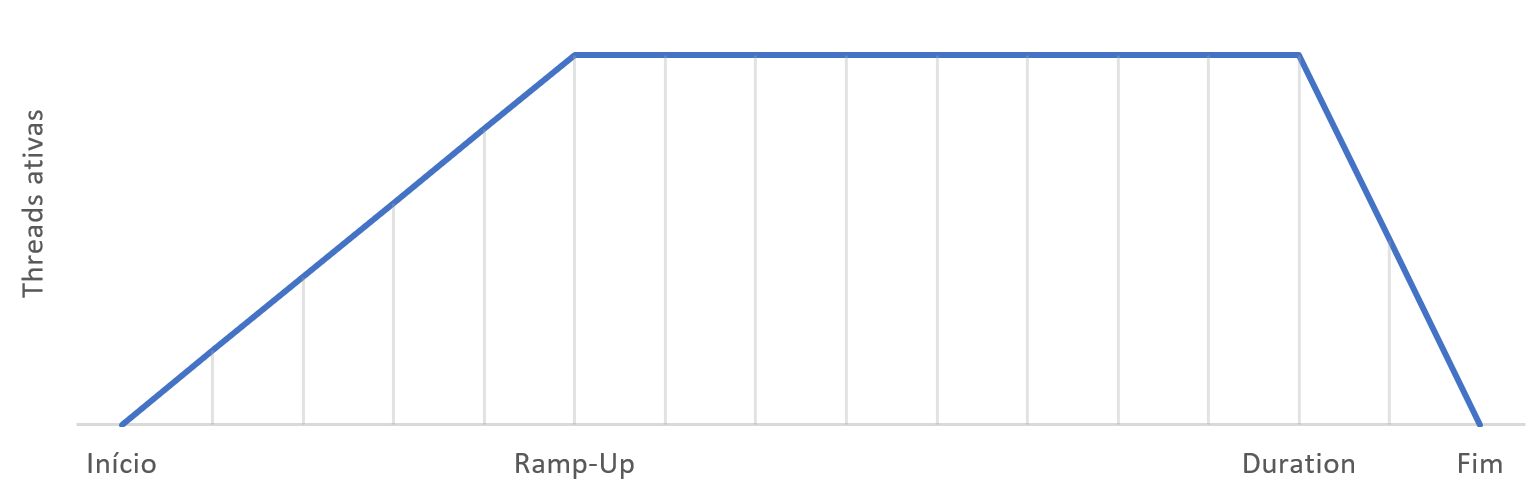
\includegraphics[width=1\textwidth]{images/Testes/ramp_up_test.PNG}
    \caption{Quantidade de \textit{threads} ativas durante a execução do \textit{script} de \textbf{teste 2}.}
    \label{fig:jmeter_ramp_up_test}
\end{figure}

\subsubsection{Parametrização dos Testes}
Com a ferramenta \texttt{Apache JMeter} é possível definir grupos de \textit{threads}, cada uma responsável pela execução de um conjunto de operações (pedidos HTTP) e pelo estabelecimento dos parâmetros indicados na secção \ref{sec:ferramenta_utilizada}. Assim, optou-se por realizar um conjunto de teste considerados fundamentais na aplicação desenvolvida, sendo estes os seguintes: 
\begin{itemize}
    \item Registo e consulta de dados pessoais:
    \begin{itemize}
        \item \texttt{Registo do utilizador}: Pedido HTTP POST ao \textit{endpoint} \texttt{users};
        \item \texttt{Login}: Pedido HTTP POST ao \textit{endpoint} \texttt{authentication};
        \item \texttt{Consulta dos dados pessoais}: Pedido HTTP GET ao \textit{endpoint} \texttt{users};
        \item \texttt{Logout}: Pedido HTTP POST ao \textit{endpoint} \texttt{authentication}.
    \end{itemize}
    \item Pesquisa s/ \textit{login}:
    \begin{itemize}
        \item \texttt{Pesquisa}: Pedido HTTP GET ao \textit{endpoint} \texttt{search}.
    \end{itemize}
    \item Pesquisa c/ \textit{login}:
    \begin{itemize}
        \item \texttt{Login}: Pedido HTTP POST ao \textit{endpoint} \texttt{authentication};
        \item \texttt{Pesquisa}: Pedido HTTP GET ao \textit{endpoint} \texttt{search};
        \item \texttt{Logout}: Pedido HTTP POST ao \textit{endpoint} \texttt{authentication}.
    \end{itemize}
    \item Editar dados pessoais e consultar estatísticas:
    \begin{itemize}
        \item \texttt{Login}: Pedido HTTP POST ao \textit{endpoint} \texttt{authentication};
        \item \texttt{Consulta dos dados pessoais}: Pedido HTTP GET ao \textit{endpoint} \texttt{users};
        \item \texttt{Edição dos dados pessoais}: Pedido HTTP PUT ao \textit{endpoint} \texttt{users};
        \item \texttt{Consulta de estatísticas}: Pedido HTTP GET ao \textit{endpoint} \texttt{statistics};
        \item \texttt{Logout}: Pedido HTTP POST ao \textit{endpoint} \texttt{authentication}.
    \end{itemize}
\end{itemize}

Todos os grupos de \textit{threads} previamente referidos exigem a utilização de um conjunto de dados pré-definido. De forma a evitar o envio repetido dos mesmos dados, criaram-se \textit{data sets} em ficheiros \texttt{csv}, que são importados para o \texttt{Apache JMeter} sendo que cada coluna desse ficheiro corresponde a uma variável a ser utilizada nos pedidos efetuados. Para os vários pedidos, as linhas destes ficheiros \texttt{csv} são percorridas sequencialmente.

Uma vez que alguns dos pedidos efetuados requeriam a autenticação do utilizador, que é efetuada através de \textit{cookies}, foi necessário o armazenamento de uma variável especial (\texttt{JSESSIONID}), recolhida aquando da receção da resposta do pedido de \textit{login}. Para a extração desta variável, bem como outras, utilizou-se o \textit{Regular Expression Extractor} do \texttt{Apache JMeter}.

Relativamente aos parâmetros referidos na secção \ref{sec:ferramenta_utilizada}, definiram-se como testes a executar os apresentados nas tabelas \ref{tab:param1} e \ref{tab:param2}.

\begin{table}[H]
\centering
\caption{Parâmetros para os vários testes realizados com 1 servidor aplicacional.}
\label{tab:param1}
\begin{tabular}{ccccc}
\hline
\rowcolor[HTML]{EFEFEF} 
\textbf{\begin{tabular}[c]{@{}c@{}}Tipo do\\ Teste\end{tabular}} & \textit{\textbf{\begin{tabular}[c]{@{}c@{}}Number of\\ threads\end{tabular}}} & \textit{\textbf{\begin{tabular}[c]{@{}c@{}}Ramp-Up\\ Period (s)\end{tabular}}} & \textit{\textbf{Loop Count}}       & \textit{\textbf{\begin{tabular}[c]{@{}c@{}}Scheduler\\ Duration\end{tabular}}} \\ \hline
                                                                 & 400                                                                           &                                                                                &                                    &                                                                                \\
                                                                 & 700                                                                           &                                                                                &                                    &                                                                                \\
\multirow{-3}{*}{1}                                              & 750                                                                           & \multirow{-3}{*}{120}                                                          & \multirow{-3}{*}{2}                & \multirow{-3}{*}{--}                                                            \\ \hline
                                                                 & 50                                                                            &                                                                                &                                    &                                                                                \\
                                                                 & 30                                                                            &                                                                                &                                    &                                                                                \\
\multirow{-3}{*}{2}                                              & 20                                                                            & \multirow{-3}{*}{50}                                                           & \multirow{-3}{*}{\textit{Forever}} & \multirow{-3}{*}{120}                                                          \\ \hline
\end{tabular}
\end{table}


\begin{table}[H]
\centering
\caption{Parâmetros para os vários testes realizados com 2 servidores aplicacionais.}
\label{tab:param2}
\begin{tabular}{ccccc}
\hline
\rowcolor[HTML]{EFEFEF} 
\textbf{\begin{tabular}[c]{@{}c@{}}Tipo do\\ Teste\end{tabular}} & \textit{\textbf{\begin{tabular}[c]{@{}c@{}}Number of\\ threads\end{tabular}}} & \textit{\textbf{\begin{tabular}[c]{@{}c@{}}Ramp-Up\\ Period (s)\end{tabular}}} & \textit{\textbf{Loop Count}}       & \textit{\textbf{\begin{tabular}[c]{@{}c@{}}Scheduler\\ Duration\end{tabular}}} \\ \hline
                                                                 & 100                                                                           &                                                                                &                                    &                                                                                \\
\multirow{-2}{*}{1}                                              & 400                                                                           & \multirow{-2}{*}{120}                                                          & \multirow{-2}{*}{2}                & \multirow{-2}{*}{-}                                                            \\ \hline
                                                                 & 100                                                                           &                                                                                &                                    &                                                                                \\
\multirow{-2}{*}{2}                                              & 50                                                                            & \multirow{-2}{*}{50}                                                           & \multirow{-2}{*}{\textit{Forever}} & \multirow{-2}{*}{120}                                                          \\ \hline
\end{tabular}
\end{table}


\subsubsection{Dificuldades}

As maiores dificuldades encontradas nesta fase de avaliação de performance foram a familiarização com a ferramenta de teste de carga, uma vez que nunca nenhum elemento do grupo tinha lidado com uma semelhante previamente, bem como o estabelecimento de toda a infraestrutura e o \textit{deployment} da aplicação (\texttt{Docker}).

Relativamente à ferramenta \texttt{Apache JMeter}, sobressaiu-se a dificuldade de aprendizagem de passagem de parâmetros à mesma, mais concretamente, a autenticação (\textit{cookie}), extração de variáveis e pedidos HTTP com parâmetros. 

Por fim, é de se referir o surgimento de erros relacionados com a concorrência e utilização de \texttt{Hibernate}, que apenas foram detetados nesta fase. Primariamente percebeu-se a necessidade de aumentar o tamanho da \textit{pool} do \texttt{Hibernate} de conexões à base de dados, tendo este processo sido efetuado com recurso à biblioteca \texttt{C3P0}. Para além disso, continuaram-se a detetar alguns erros inerentes à possibilidade de execução concorrente, como por exemplo, a ocorrência de \textit{rolbacks}.

\subsubsection{Resultados}

Com a realização dos testes definidos na tabela \ref{tab:param1} e \ref{tab:param2}, obtiveram-se os resultados apresentados de seguida, nas secções \ref{sec:app1} e \ref{sec:app2} respetivamente. 

Salienta-se que em todos os testes apresentados se verifica uma quantidade de \textit{threads} ativas inicial bastante elevado, relativamente ao resto da execução, devido a esta ser uma fase em que o servidor aplicacional tem de criar sessões do \texttt{Hibernate} (conexões à base de dados), bem como instâncias de EJBs e \textit{Servlets}. Assim que estas instanciações terminem, o servidor aplicacional adquire uma maior capacidade de resposta.

\newpage
\paragraph{Arquitetura com um Servidor Aplicacional}\label{sec:app1}

\vspace{0.5cm}
\noindent\textbf{Teste do tipo 1 com 400 utilizadores virtuais:}
%Teste 400
%throughput: 42,10s
%response: 82ms

Neste teste obteve-se um débito de 42,10 operações por segundo e um tempo de resposta médio de 82 milissegundos. Para além disso, obteve-se uma quantidade de \textit{threads} ativas aceitáveis (geralmente inferior a 2 \textit{threads}, após estabilizar), como se pode verificar através da figura \ref{fig:3PC_400_threads}. Adicionalmente, verificou-se que a taxa de insucesso na receção de resposta encontra-se na ordem dos 3,15\%. 


\begin{figure}[H]
    \centering
    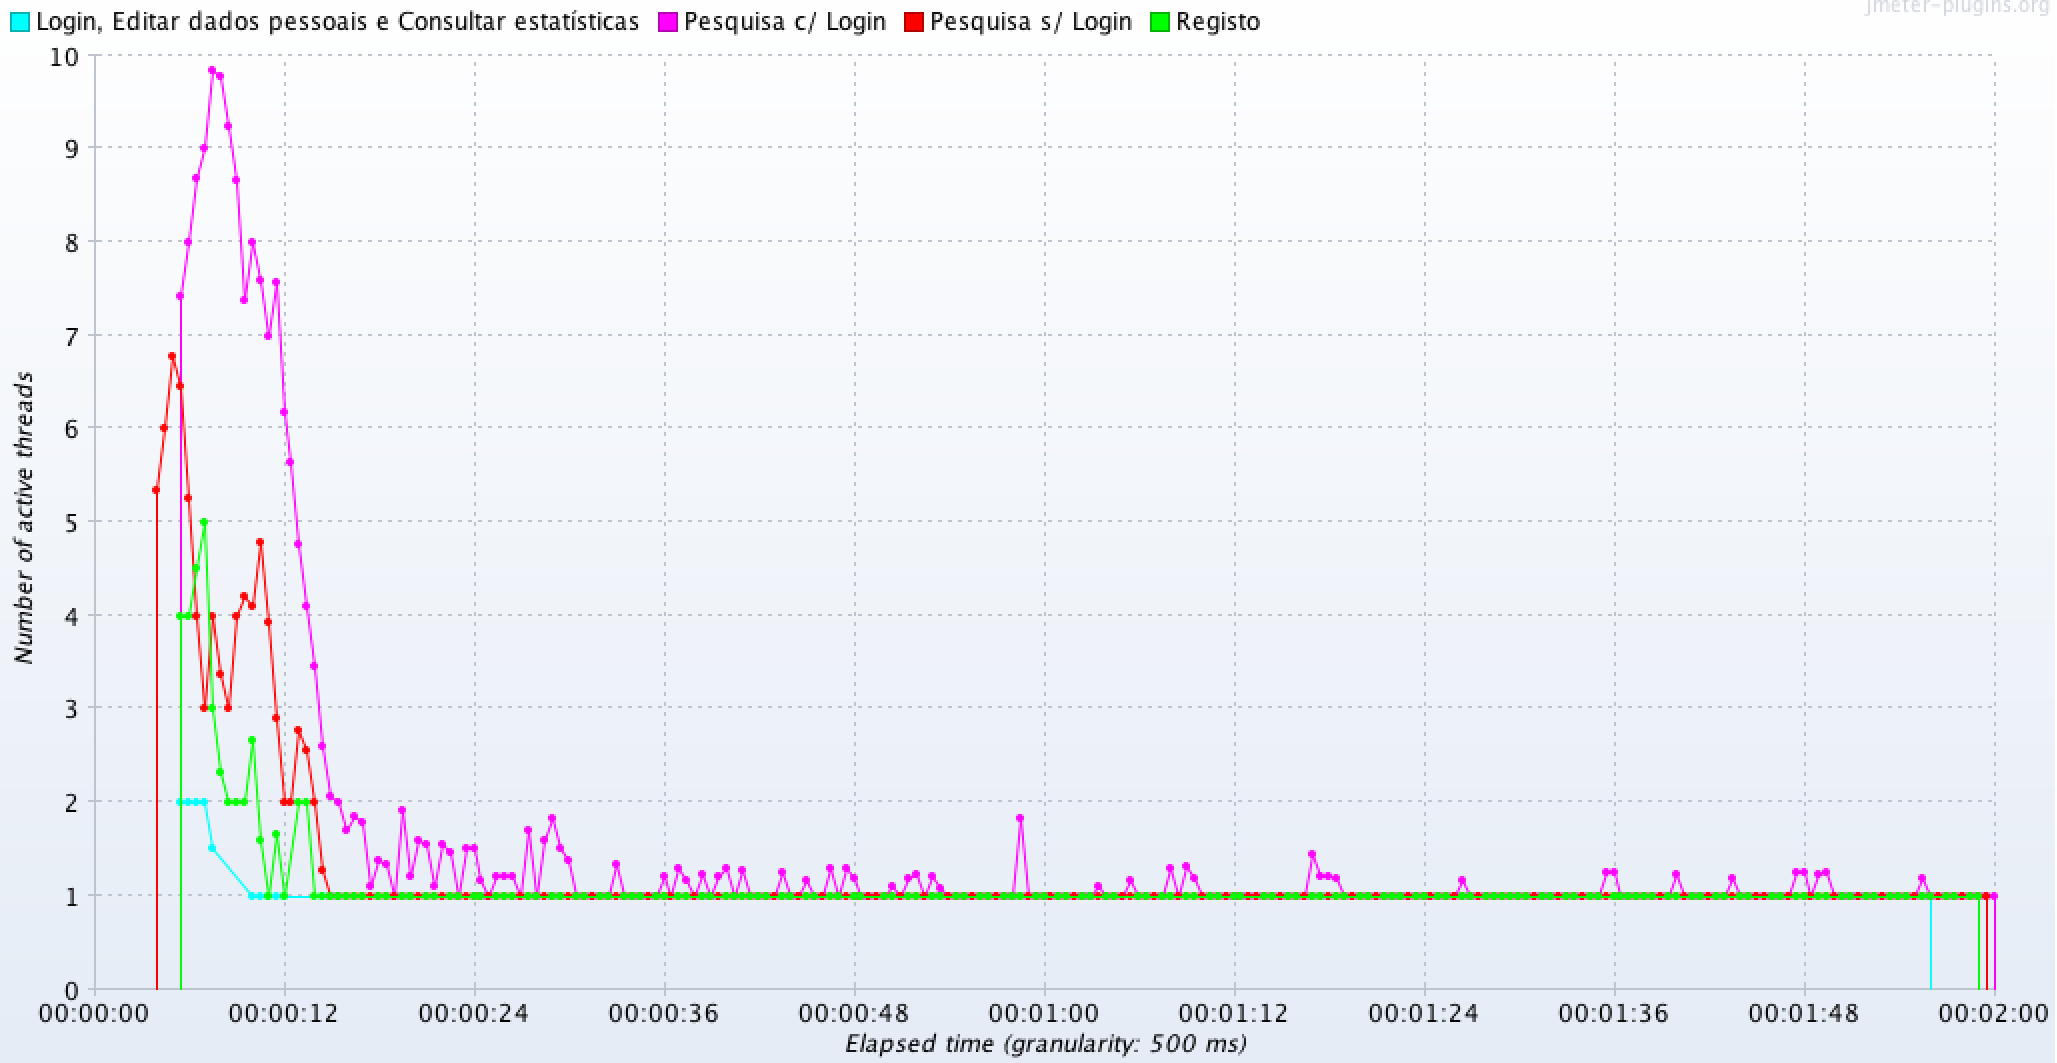
\includegraphics[width=1\textwidth]{images/Testes/3PC_400T.png}
    \caption{Quantidade de \textit{threads} ativas ao longo do tempo, para o teste do tipo \textbf{1} com 400 utilizadores virtuais.}
    \label{fig:3PC_400_threads}
\end{figure}

\begin{figure}[H]
    \centering
    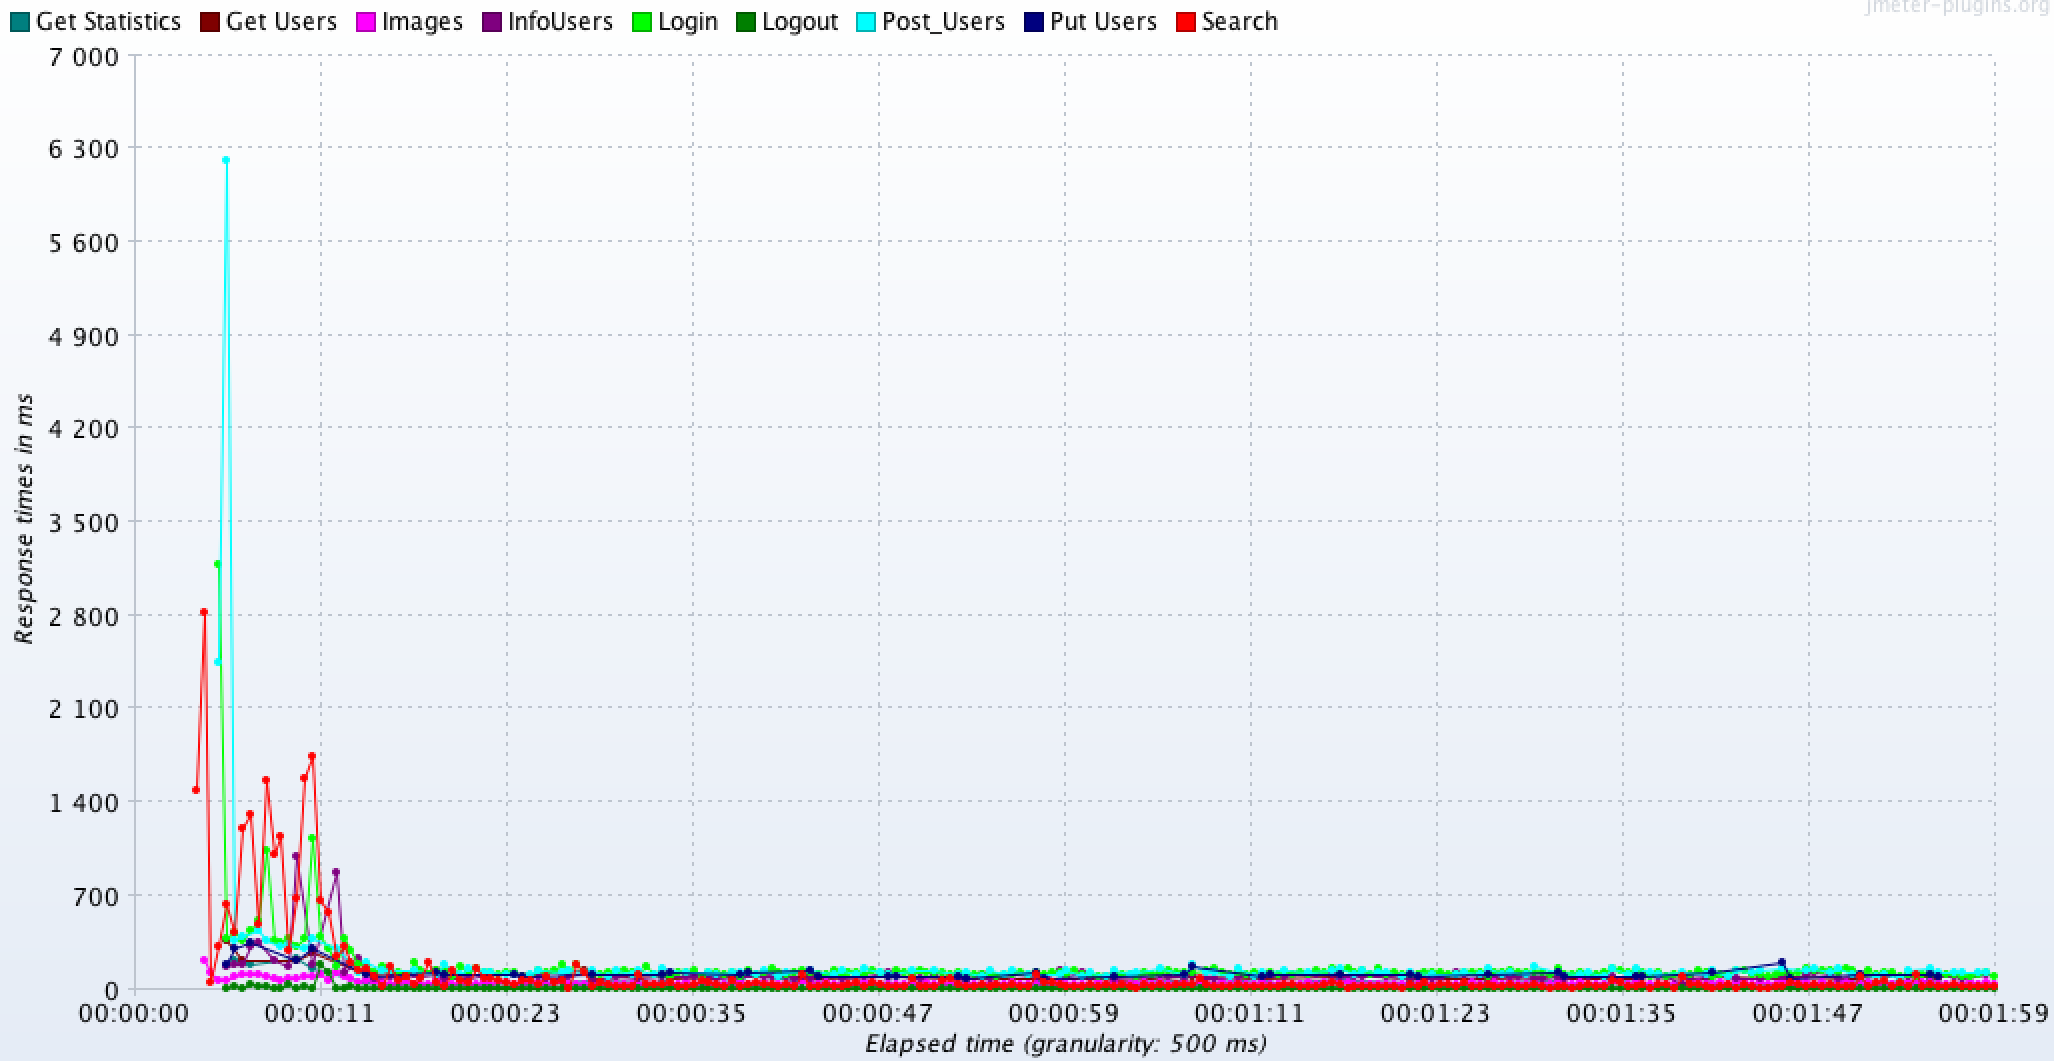
\includegraphics[width=1\textwidth]{images/Testes/3PC_400R.png}
    \caption{Tempo de resposta aos pedidos efetuados ao longo do tempo, para o teste do tipo \textbf{1} com 400 utilizadores virtuais.}
    \label{fig:3PC_400_response}
\end{figure}

\begin{table}[H]
\centering
\caption{Quantidade de sucessos e insucessos, bem com percentagem de insucesso, para o teste do tipo \textbf{1} com 400 utilizadores virtuais.}
\begin{tabular}{cccc}
\hline
\rowcolor[HTML]{EFEFEF} 
\textbf{Thread-Group}                  & \textbf{Sucesso} & \textbf{Insucesso} & \textbf{\% Insucesso} \\ \hline
\textbf{pesquisa c/ login}             & 2305             & 95                 & 3,96\%                \\
\textbf{pesquisa s/ login}             & 1744             & 56                 & 3,11\%                \\
\textbf{registo}                       & 593              & 7                  & 1,17\%                \\
\textbf{editar info pessoais}          & 249              & 1                  & 0,40\%                \\ \hline
\cellcolor[HTML]{EFEFEF}\textbf{Total} & 4891             & 159                & 3,15\%                \\ \hline
\end{tabular}
\end{table}

Considera-se que estes resultados são bastantes positivos, pelo que se optou por aumentar o número de utilizadores virtuais para este tipo de teste.

\vspace{0.5cm}
\noindent\textbf{Teste do tipo 1 com 700 utilizadores virtuais:}
%Teste 700
%throughput: 71,58s
%response: 170ms

Neste teste obteve-se um débito de 71,58 operações por segundo e um tempo de resposta médio de 170 milissegundos. Para além disso, obteve-se ainda uma quantidade de \textit{threads} ativas aceitáveis (geralmente inferior a 3 \textit{threads}, após estabilizar), como se pode verificar através da figura \ref{fig:3PC_700_threads}. Adicionalmente, verificou-se que a taxa de insucesso na receção de resposta encontra-se na ordem dos 3,77\%. 

\begin{figure}[H]
    \centering
    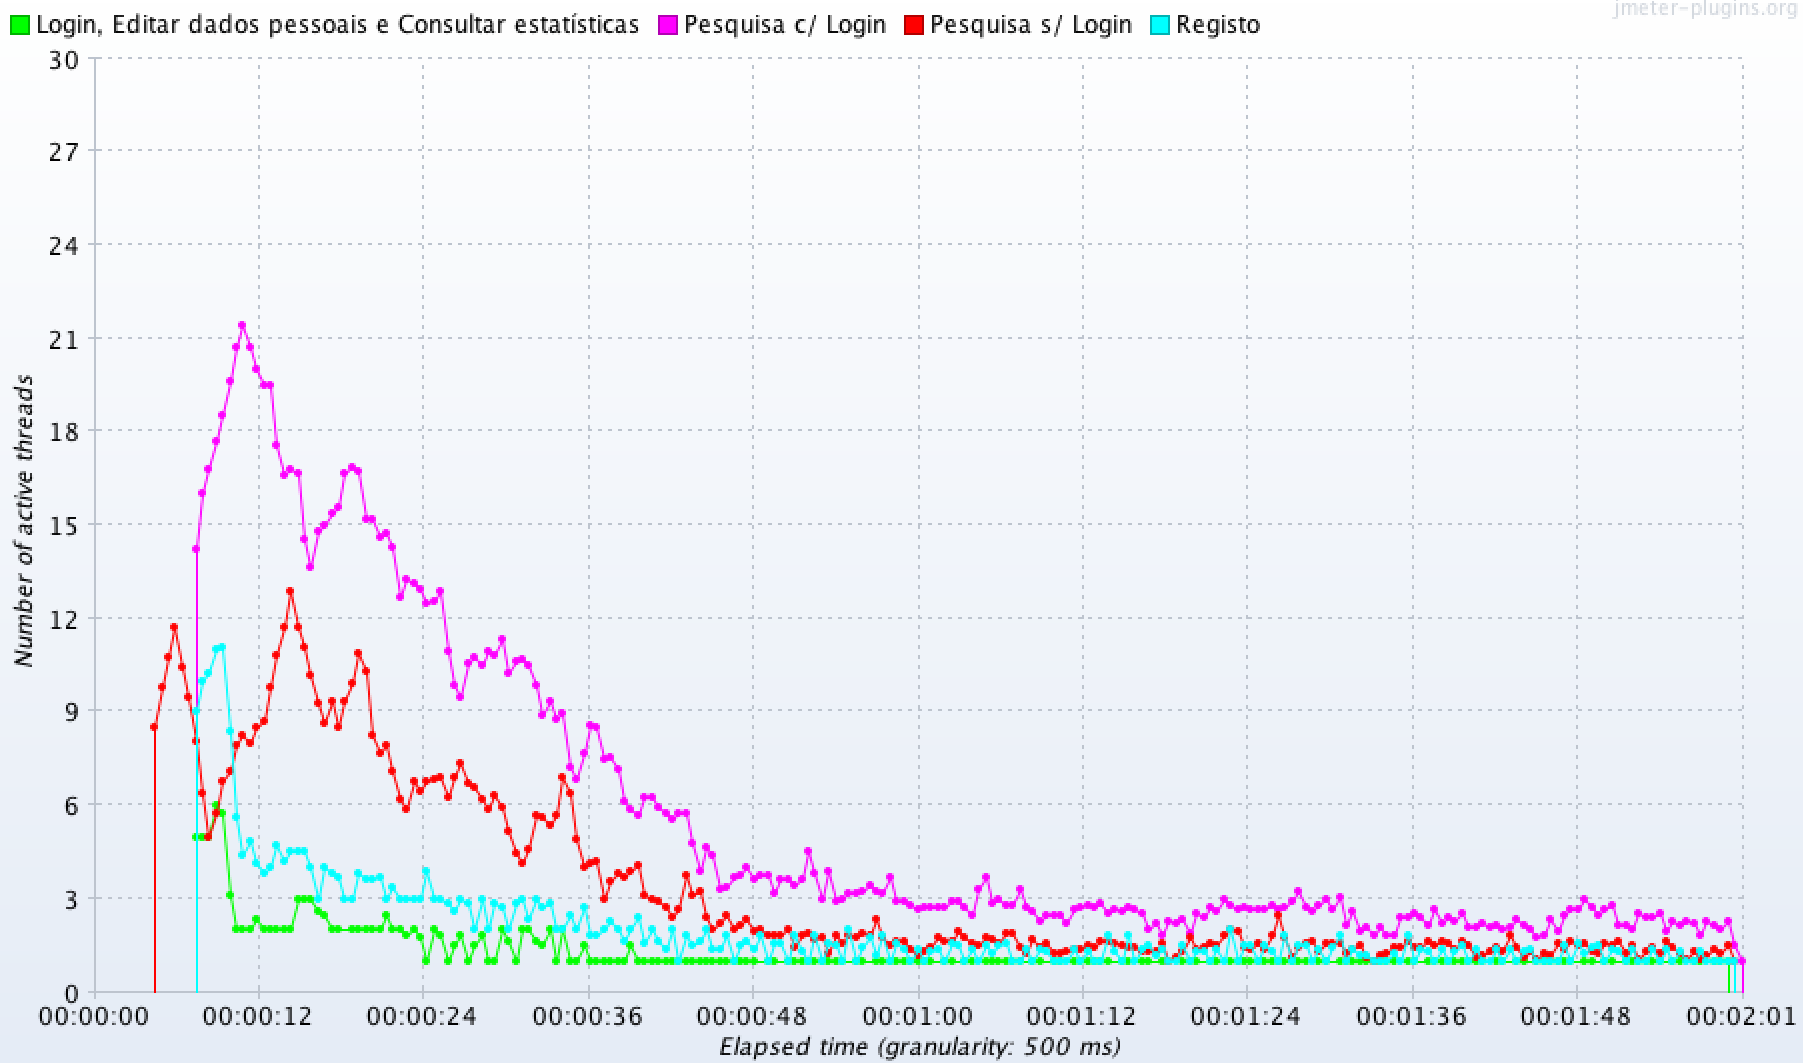
\includegraphics[width=1\textwidth]{images/Testes/3PC_700T.png}
    \caption{Quantidade de \textit{threads} ativas ao longo do tempo, para o teste do tipo \textbf{1} com 700 utilizadores virtuais.}
    \label{fig:3PC_700_threads}
\end{figure}

\begin{figure}[H]
    \centering
    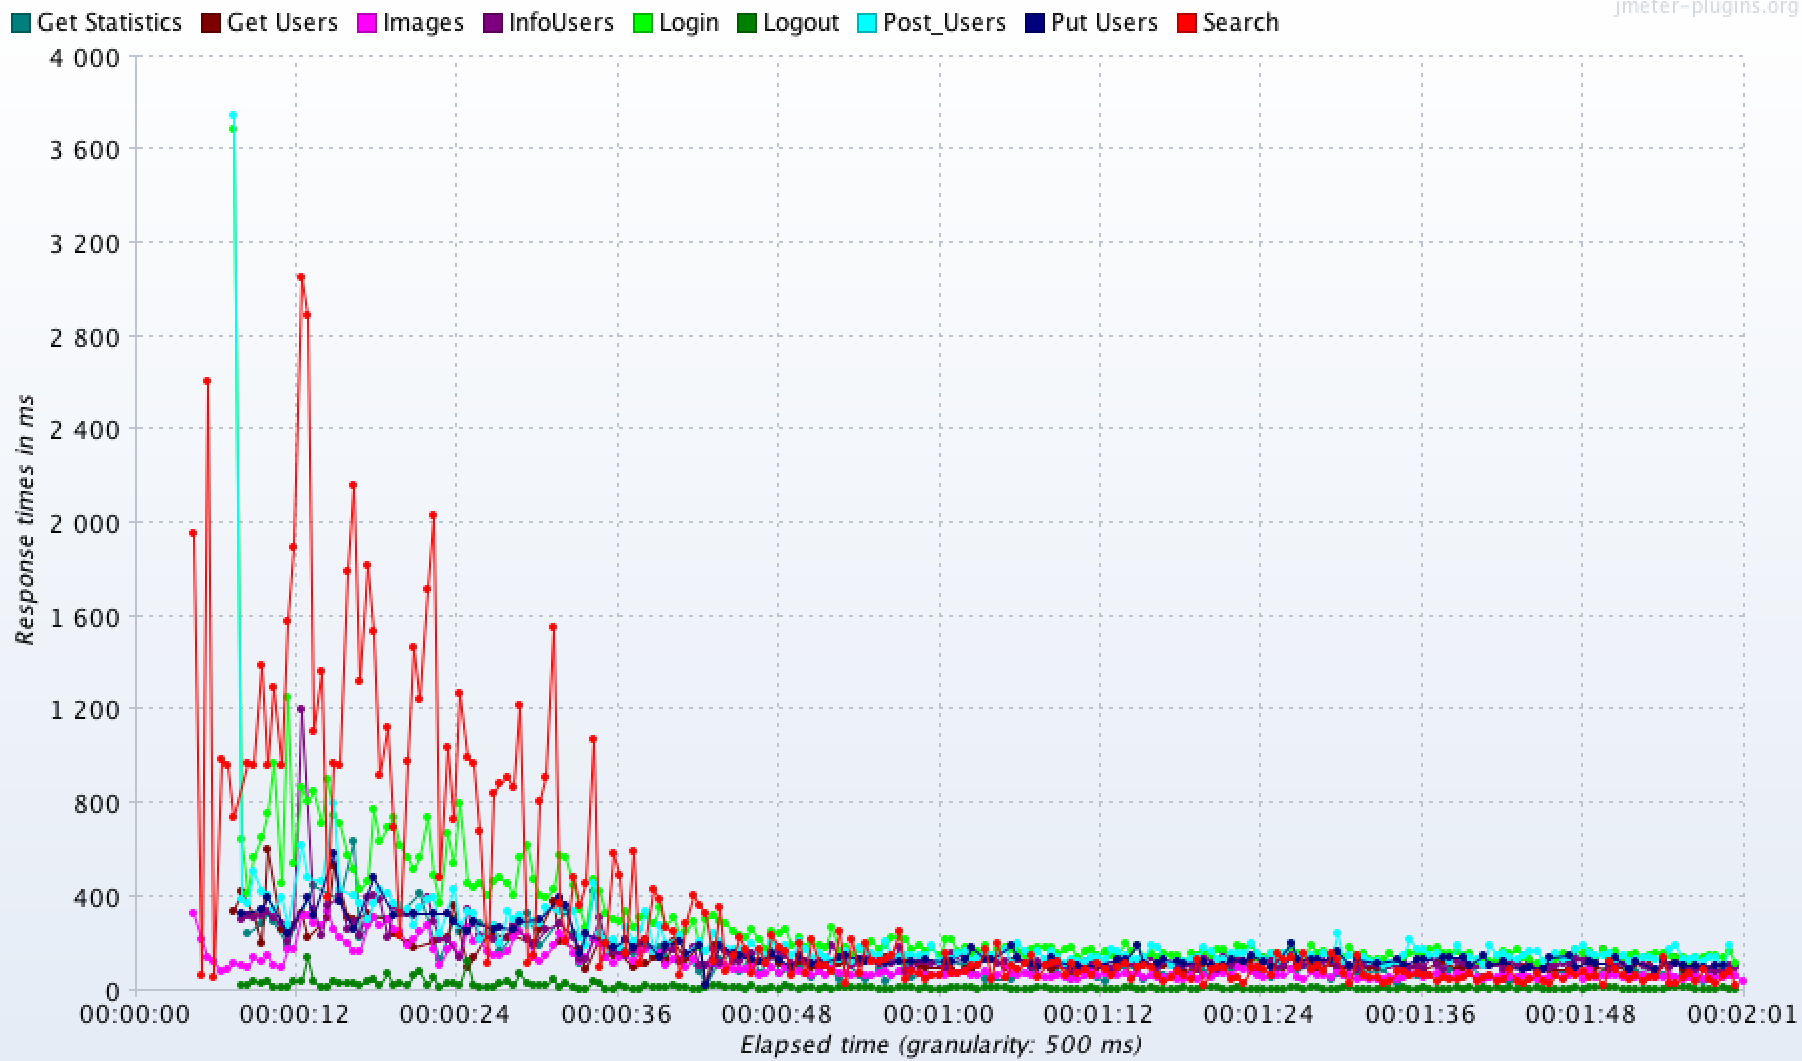
\includegraphics[width=1\textwidth]{images/Testes/3PC_700R.png}
    \caption{Tempo de resposta aos pedidos efetuados ao longo do tempo, para o teste do tipo \textbf{1} com 700 utilizadores virtuais.}
    \label{fig:3PC_700_response}
\end{figure}

\begin{table}[H]
\centering
\caption{Quantidade de sucessos e insucessos, bem com percentagem de insucesso, para o teste do tipo \textbf{1} com 700 utilizadores virtuais.}
\begin{tabular}{cccc}
\hline
\rowcolor[HTML]{EFEFEF} 
\textbf{Thread-Group}                  & \textbf{Sucesso} & \textbf{Insucesso} & \textbf{\% Insucesso} \\ \hline
\textbf{pesquisa c/ login}             & 3625             & 215                & 5,60\%                \\
\textbf{pesquisa s/ login}             & 2786             & 94                 & 3,26\%                \\
\textbf{registo}                       & 1160             & 8                  & 0,68\%                \\
\textbf{editar info pessoais}          & 732              & 8                  & 1,08\%                \\ \hline
\cellcolor[HTML]{EFEFEF}\textbf{Total} & 8303             & 325                & 3,77\%                \\ \hline
\end{tabular}
\end{table}

Estes resultados mantêm-se ainda animadores, contudo é de se realçar que o período de tempo que o servidor aplicacional demorou a estabilizar a quantidade de pedidos respondidos aumentou consideravelmente. Este facto deve-se ao aumento da quantidade utilizadores virtuais, que se irão acumular enquanto o servidor aplicacional inicializa as instâncias de sessões do \texttt{Hibernate}, EJBs e \textit{servlets}. 

Como estes resultados continuam a ser considerados aceitáveis, mas já se revela um ligeiro acumular de \textit{threads} ativas inicialmente, optou-se por continuar a aumentar a quantidade de utilizadores virtuais, ainda que ligeiramente.

\vspace{0.5cm}
\noindent\textbf{Teste do tipo 1 com 750 utilizadores virtuais:}
%Teste 750
%throughput: 38,26185s
%response: 7279ms

Neste teste obteve-se um débito de 38,26 operações por segundo e um tempo de resposta médio de 7,28 segundos. O número de \textit{threads} ativas revela-se bastante elevado, dado que o servidor não foi capaz de lidar com a carga à qual foi submetido. Esta, por sua vez, foi-se acumulando até ao final do teste (2 minutos), momento a partir do qual os pedidos deixaram de ser efetuados e o servidor aplicacional começou a conseguir dar resposta aos previamente realizados. 

Adicionalmente, verificou-se que a taxa de insucesso na receção de resposta se encontra na ordem dos 28,68\%. 


\begin{figure}[H]
    \centering
    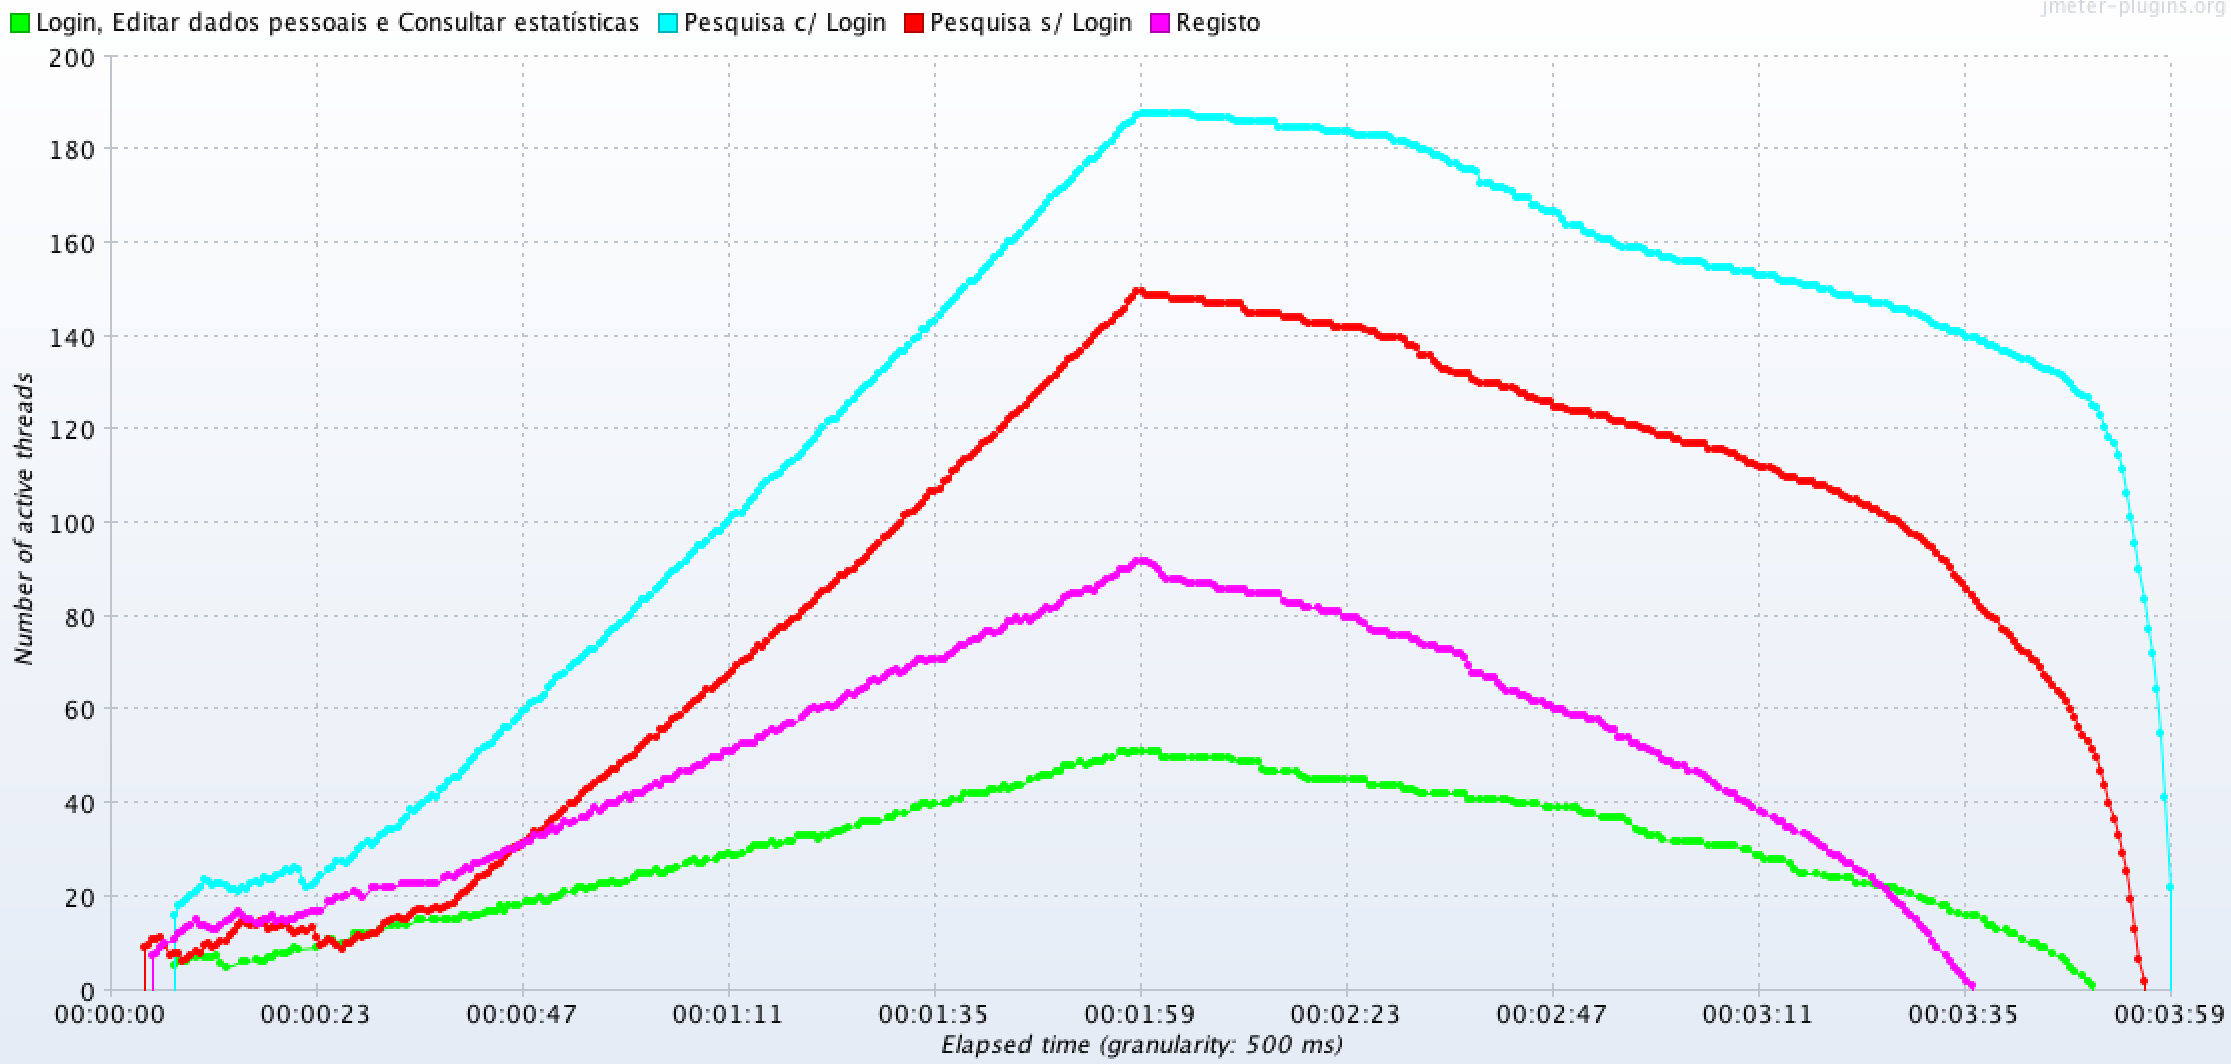
\includegraphics[width=1\textwidth]{images/Testes/3PC_750T.png}
    \caption{Quantidade de threads ativas ao longo do tempo, para o teste do tipo \textbf{1} com 750 utilizadores virtuais.}
    \label{fig:3PC_100_threads}
\end{figure}

\begin{figure}[H]
    \centering
    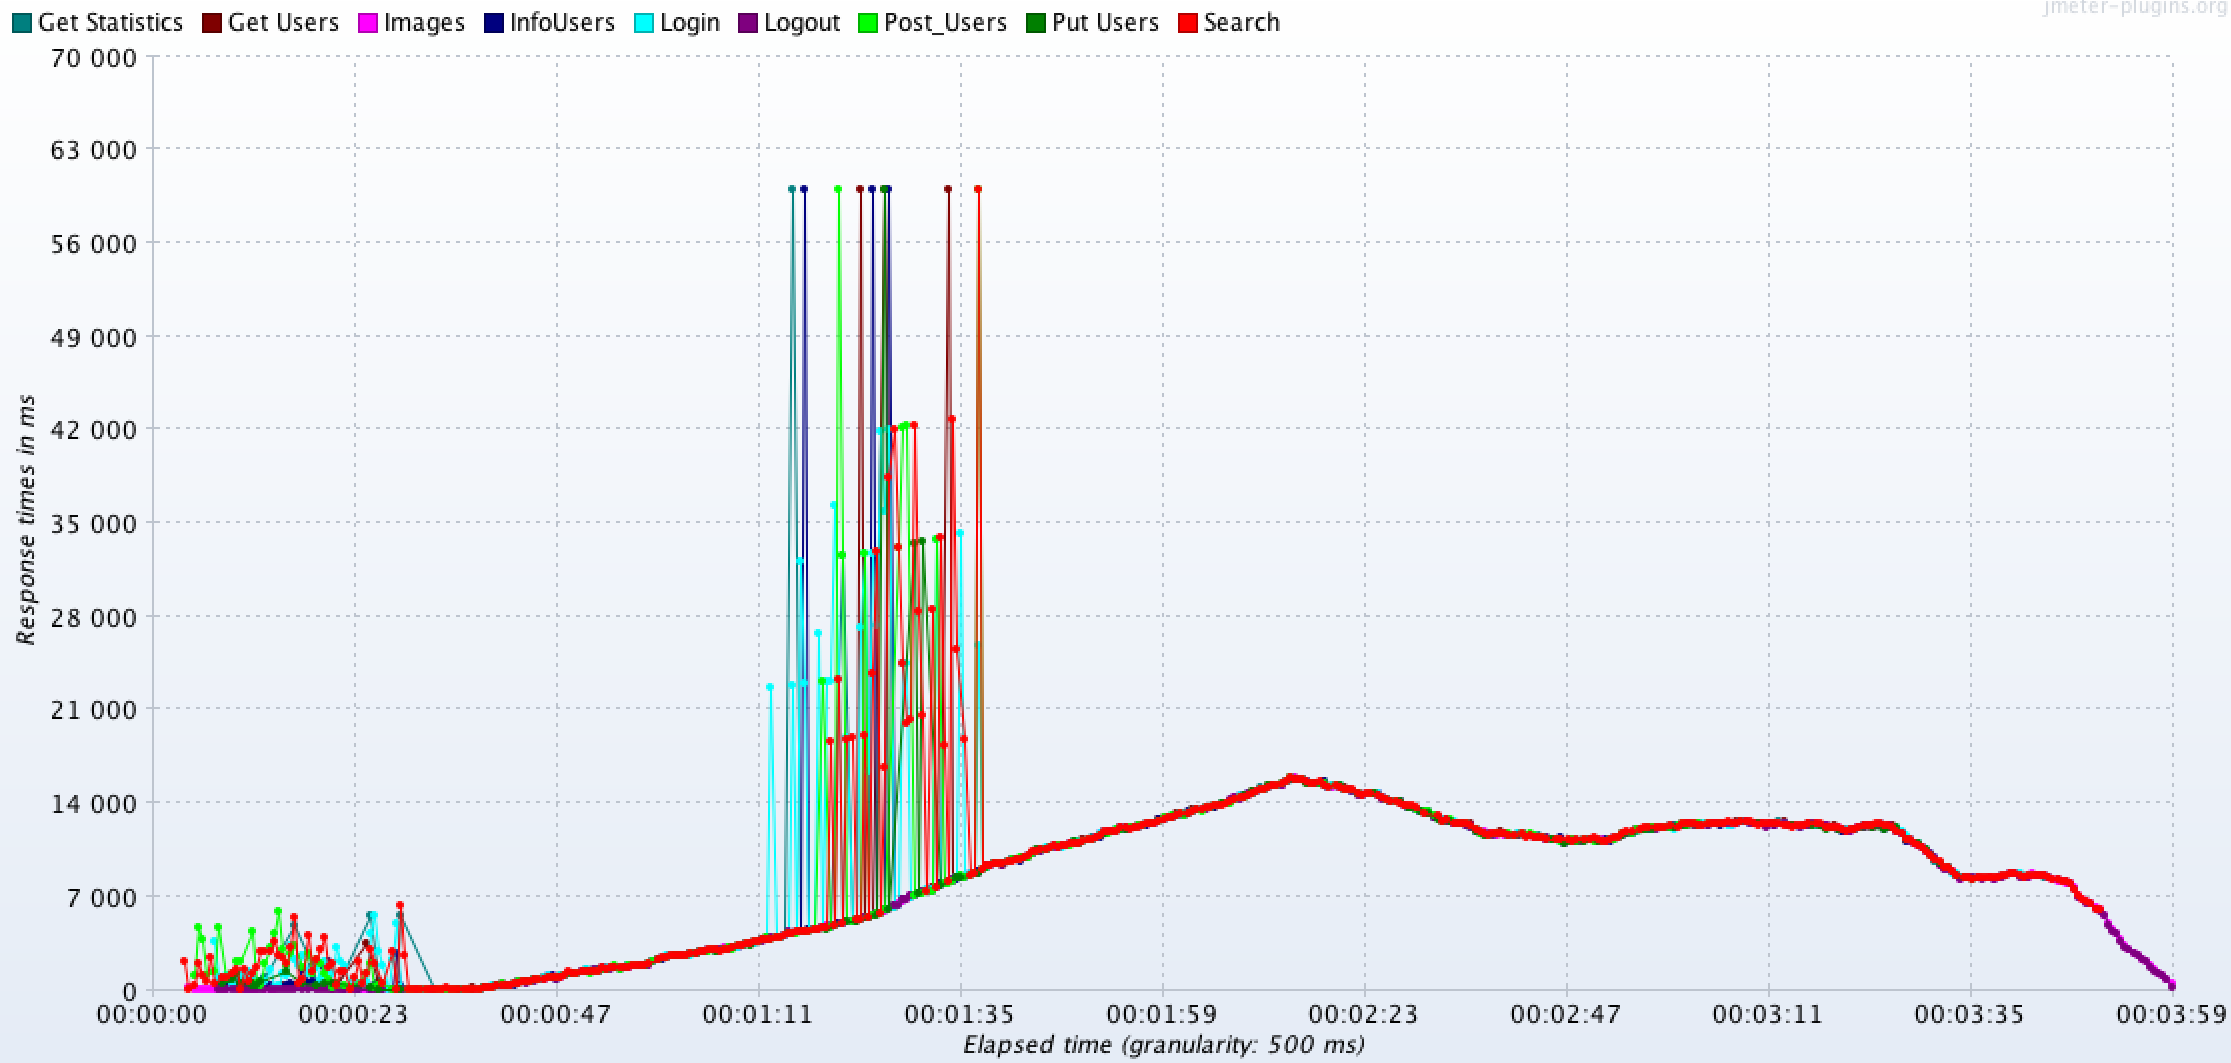
\includegraphics[width=1\textwidth]{images/Testes/3PC_750R.png}
    \caption{Tempo de resposta aos pedidos efetuados ao longo do tempo, para o teste do tipo \textbf{1} com 750 utilizadores virtuais.}
    \label{fig:3PC_100_response}
\end{figure}

\begin{table}[H]
\centering
\caption{Quantidade de sucessos e insucessos, bem com percentagem de insucesso, para o teste do tipo \textbf{1} com 750 utilizadores virtuais.}
\begin{tabular}{cccc}
\hline
\rowcolor[HTML]{EFEFEF} 
\textbf{Thread-Group}                  & \textbf{Sucesso} & \textbf{Insucesso} & \textbf{\% Insucesso} \\ \hline
\textbf{pesquisa c/ login}             & 3196             & 804                & 20,10\%               \\
\textbf{pesquisa s/ login}             & 2659             & 341                & 11,37\%               \\
\textbf{registo}                       & 179              & 1190               & 86,92\%               \\
\textbf{editar info pessoais}          & 505              & 295                & 36,88\%               \\ \hline
\cellcolor[HTML]{EFEFEF}\textbf{Total} & 6539             & 2630               & 28,68\%               \\ \hline
\end{tabular}
\end{table}

\vspace{0.5cm}
Como os resultados obtidos neste teste se revelaram negativos, considera-se que o servidor apenas é capaz de suportar 700 utilizadores virtuais para um teste do tipo 1.

\vspace{0.5cm}
\noindent\textbf{Teste do tipo 2 com 50 utilizadores virtuais:}
%Teste RU 50
%throughput: 31,79s
%response: 1053ms

Agora, com o teste do tipo 2, obteve-se um débito de 31,79 operações por segundo e um tempo de resposta médio de 1,05 segundos. Como se pode verificar no gráfico apresentado na figura \ref{fig:3PC_RU_50_threads}, a quantidade de \textit{threads} ativas vai aumentando até, aproximadamente, os 50 segundos, momento a partir do qual se mantém constante (somatório igual a 50 utilizadores virtuais, a cada instante). Relativamente ao tempo de resposta, cujo gráfico é apresentado na figura \ref{fig:3PC__RU_50_response}, verifica-se que, inicialmente, este valor é aceitável, mas que a partir do momento em que as \textit{threads} ativas atingem e se mantêm no seu valor máximo o servidor deixa de ser capaz de dar resposta a tanta carga. 

Adicionalmente, verificou-se que a taxa de insucesso na receção de resposta se encontra na ordem dos 11,94\%. 


\begin{figure}[H]
    \centering
    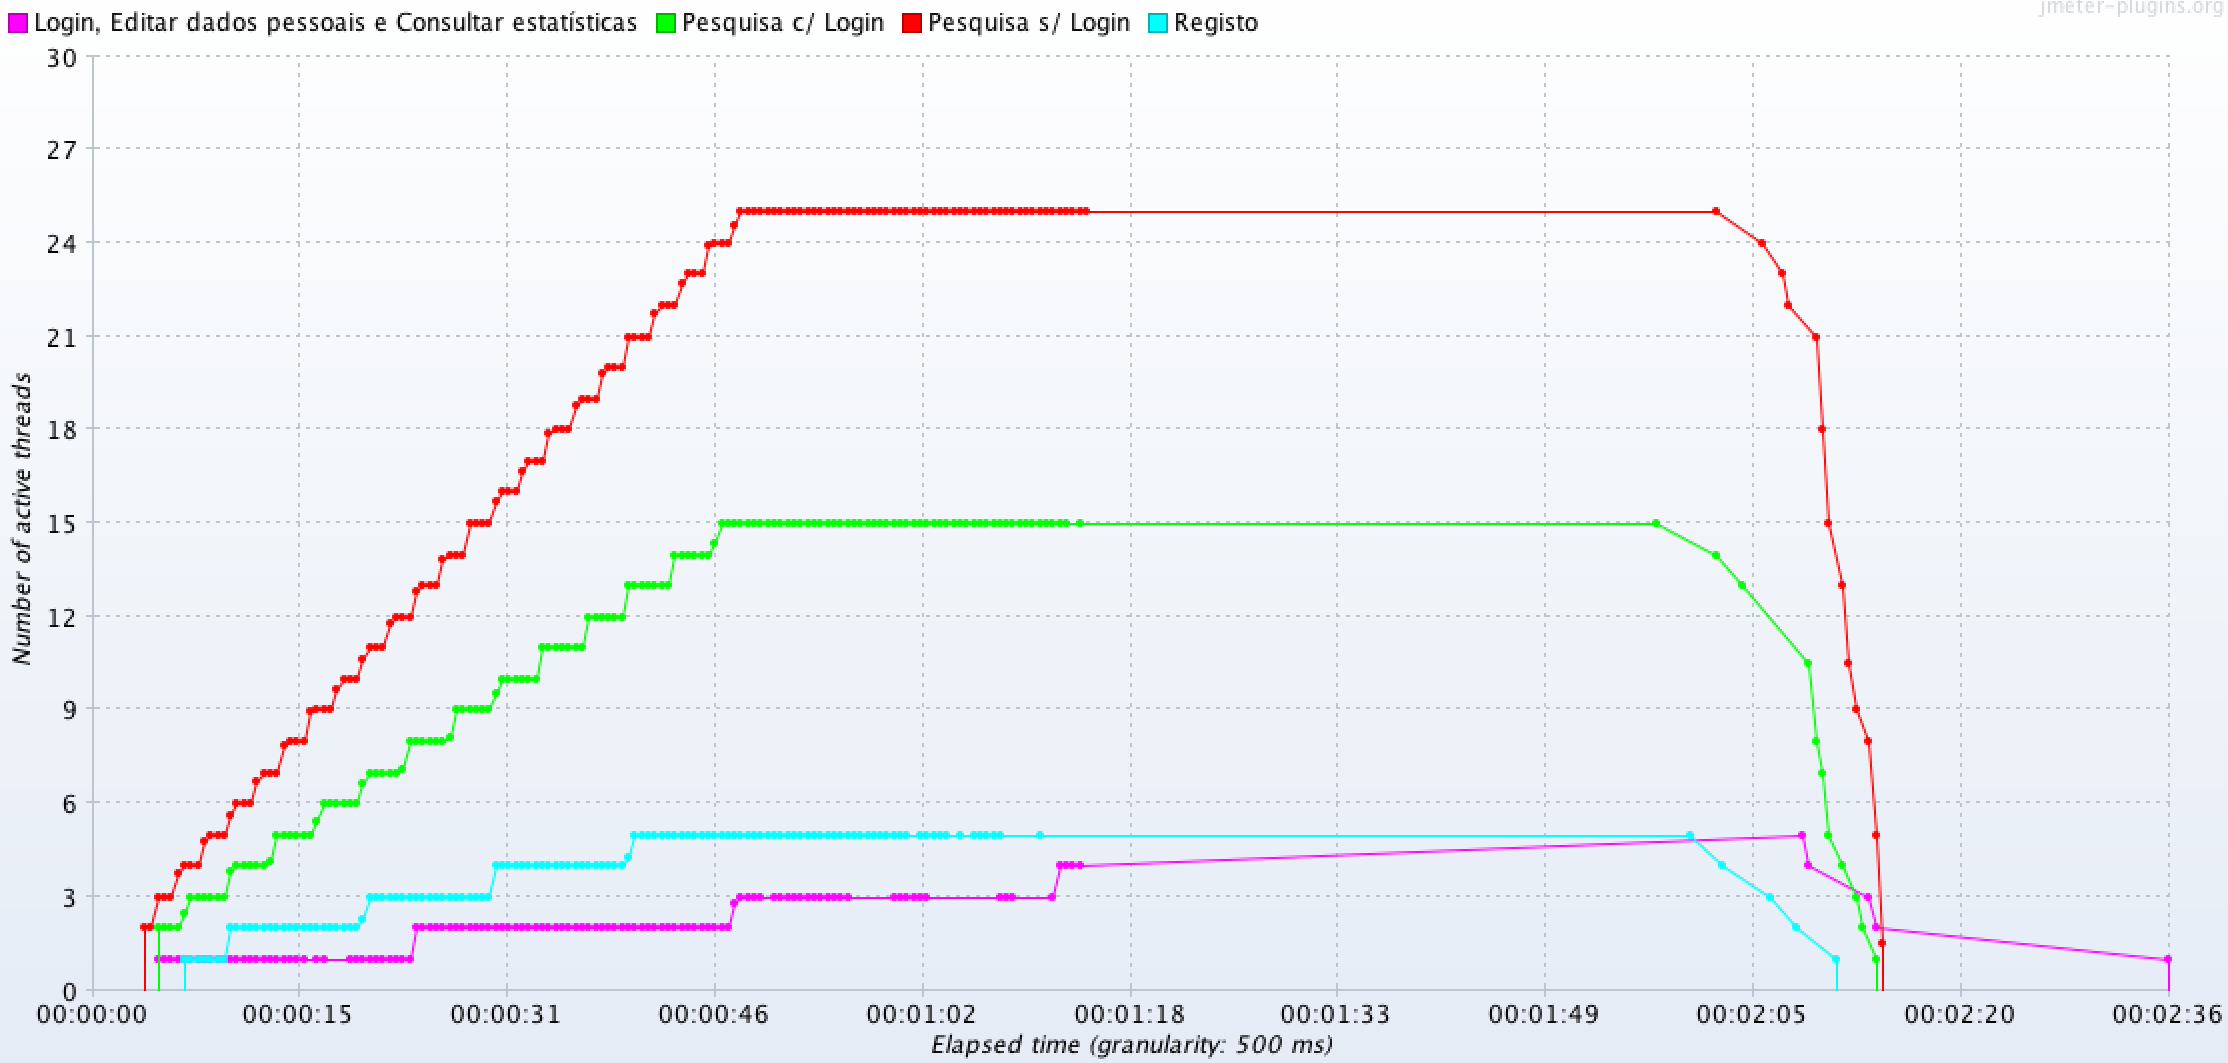
\includegraphics[width=1\textwidth]{images/Testes/3PC_RU_50T.png}
    \caption{Quantidade de \textit{threads} ativas ao longo do tempo, para o teste do tipo \textbf{2} com 50 utilizadores virtuais.}
    \label{fig:3PC_RU_50_threads}
\end{figure}

\begin{figure}[H]
    \centering
    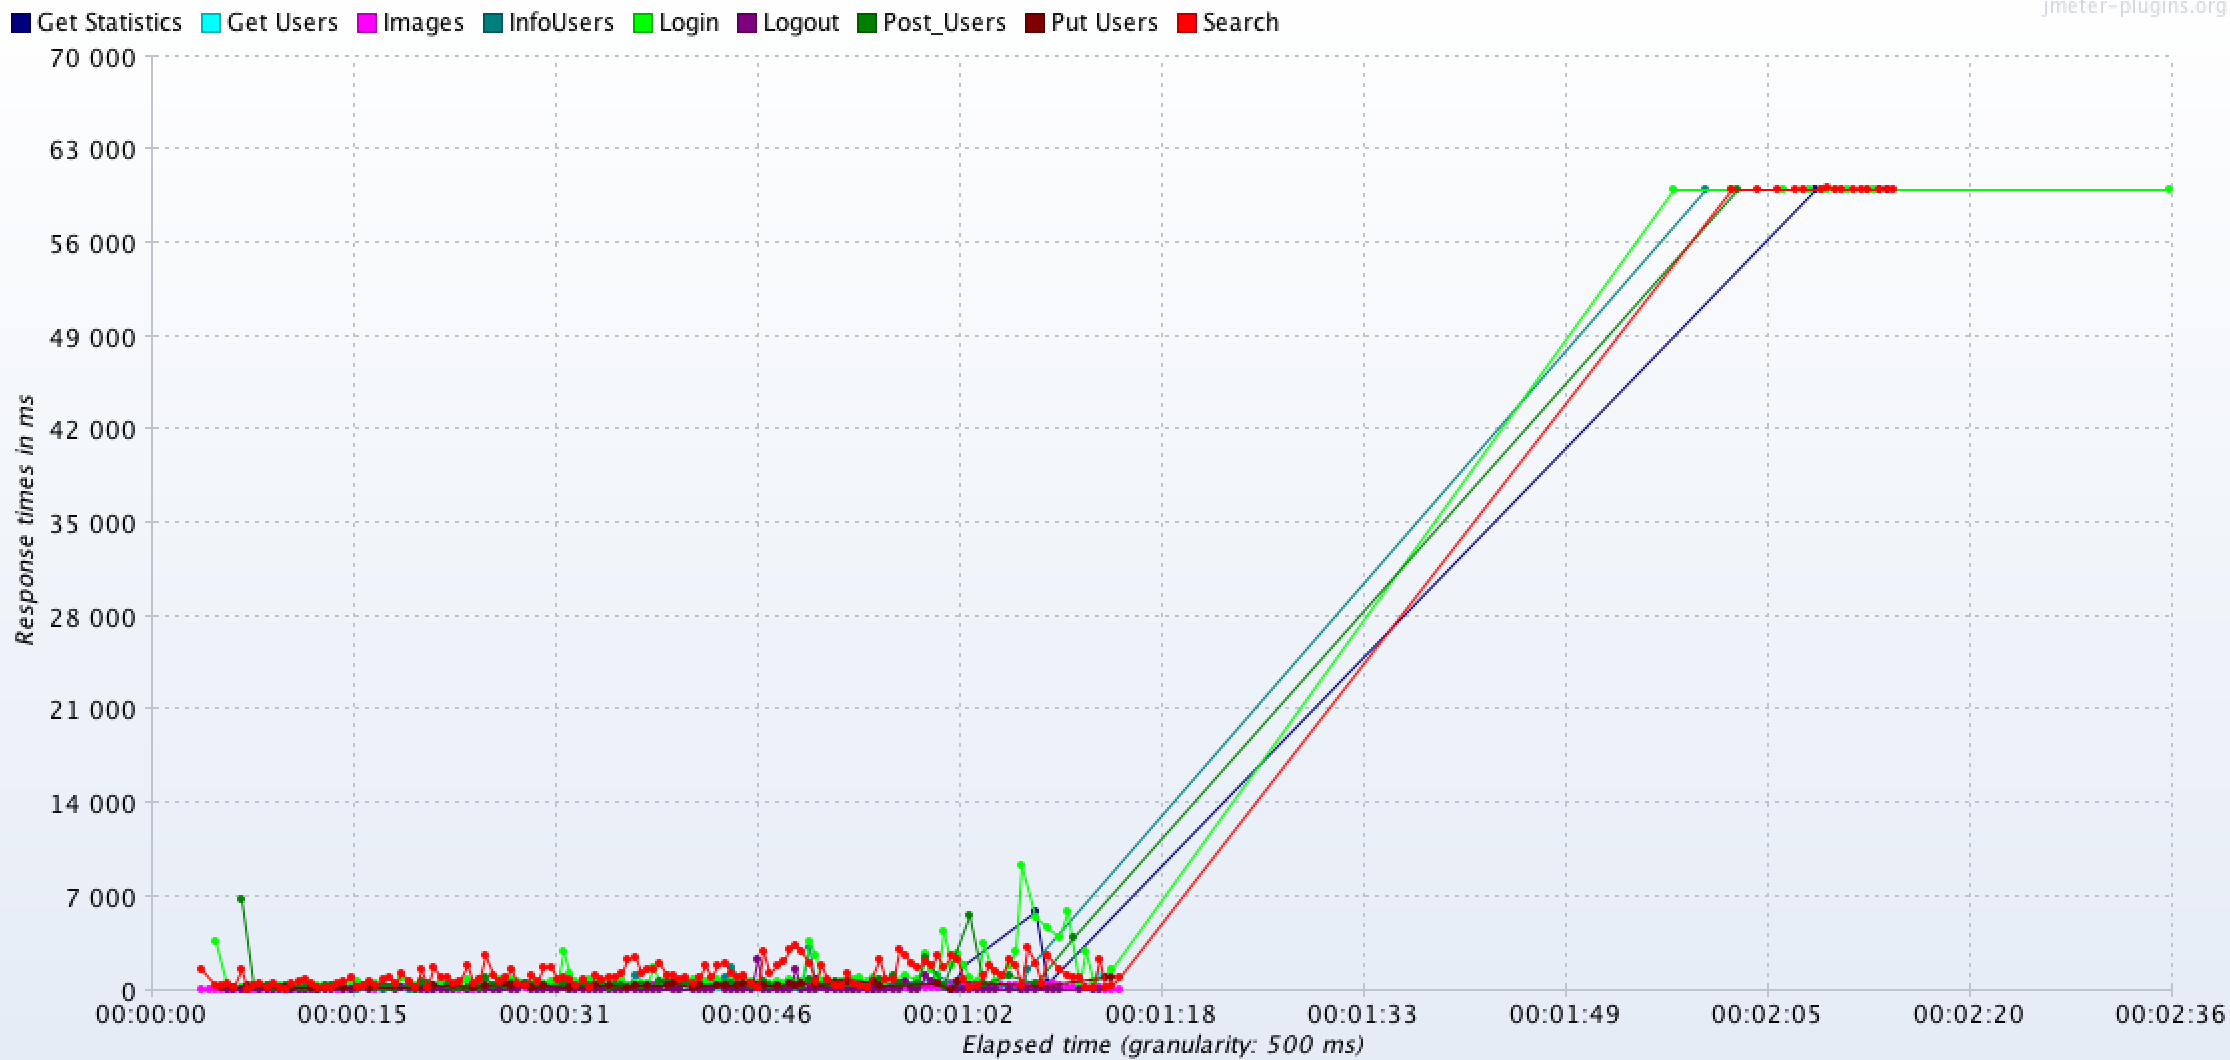
\includegraphics[width=1\textwidth]{images/Testes/3PC_RU_50R.png}
    \caption{Tempo de resposta aos pedidos efetuados ao longo do tempo, para o teste do tipo \textbf{2} com 50 utilizadores virtuais.}
    \label{fig:3PC__RU_50_response}
\end{figure}

\begin{table}[H]
\centering
\caption{Quantidade de sucessos e insucessos, bem com percentagem de insucesso, para o teste do tipo \textbf{2} com 50 utilizadores virtuais.}
\begin{tabular}{cccc}
\hline
\rowcolor[HTML]{EFEFEF} 
\textbf{Thread-Group}                  & \textbf{Sucesso} & \textbf{Insucesso} & \textbf{\% Insucesso} \\ \hline
\textbf{pesquisa c/ login}             & 1125             & 156                & 12,18\%               \\
\textbf{pesquisa s/ login}             & 2553             & 292                & 10,26\%               \\
\textbf{registo}                       & 404              & 98                 & 19,52\%               \\
\textbf{editar info pessoais}          & 283              & 46                 & 13,98\%               \\ \hline
\cellcolor[HTML]{EFEFEF}\textbf{Total} & 4365             & 592                & 11,94\%               \\ \hline
\end{tabular}
\end{table}

Assim, pode-se concluir que 50 utilizadores a efetuar pedidos ao servidor aplicacional constantemente (teste tipo 2), corresponde a uma carga demasiado elevada para o mesmo ser capaz de dar resposta. Prosseguiu-se então com uma redução de uma quantidade de utilizadores virtuais.

\vspace{0.5cm}
\noindent\textbf{Teste do tipo 2 com 30 utilizadores virtuais:}
%Teste RU 30
%throughput:45,40s
%response: 469ms

Neste teste obteve-se um débito de 45,40 operações por segundo e um tempo de resposta médio de 469 milissegundos. Apesar destes valores serem aceitáveis, o percentagem de insucesso encontra-se ainda um pouco elevado (22,03\%). 

\begin{figure}[H]
    \centering
    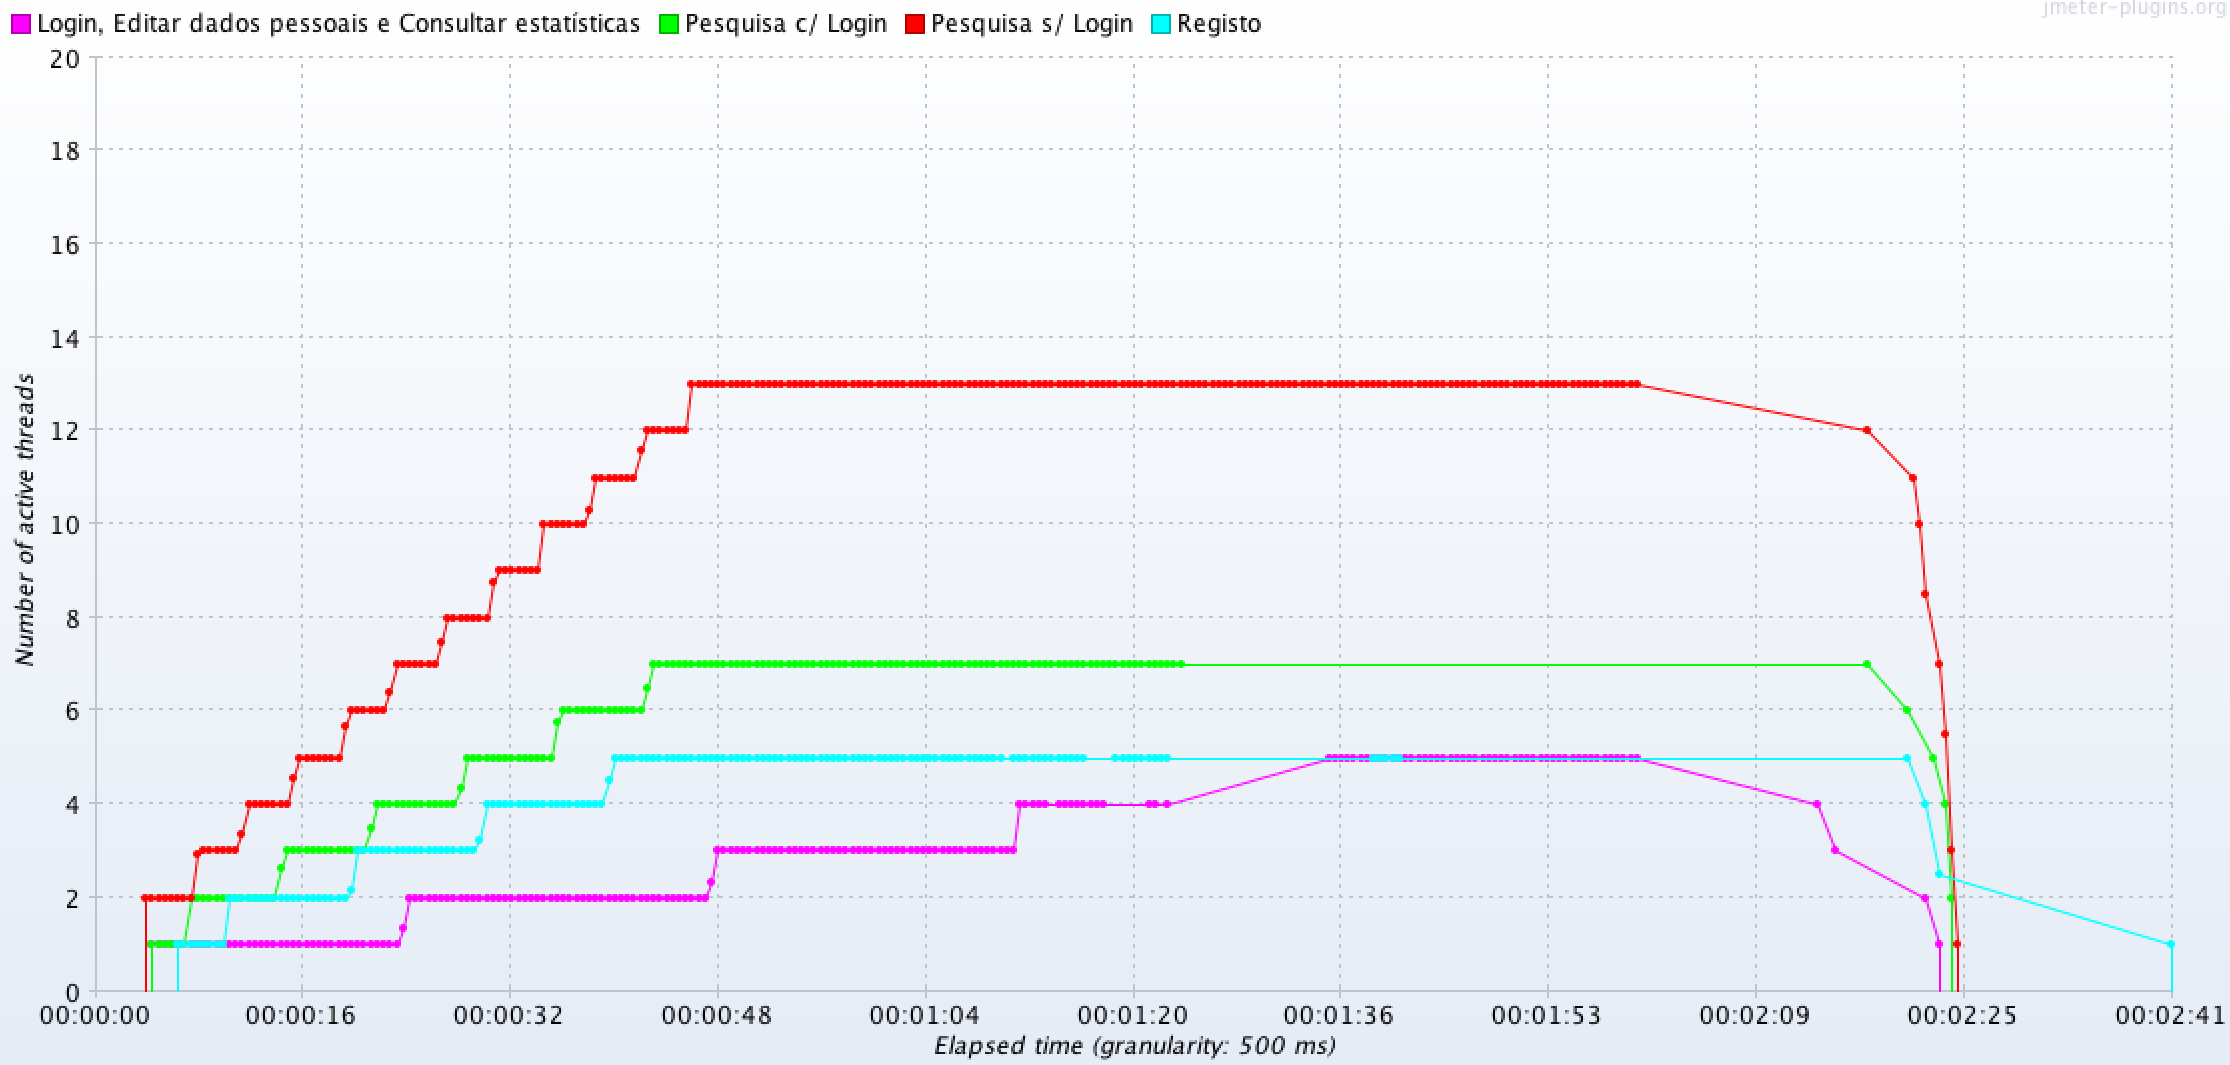
\includegraphics[width=1\textwidth]{images/Testes/3PC_RU_30T.png}
    \caption{Quantidade de \textit{threads} ativas ao longo do tempo, para o teste do tipo \textbf{2} com 30 utilizadores virtuais.}
    \label{fig:3PC_RU_30_threads}
\end{figure}

\begin{figure}[H]
    \centering
    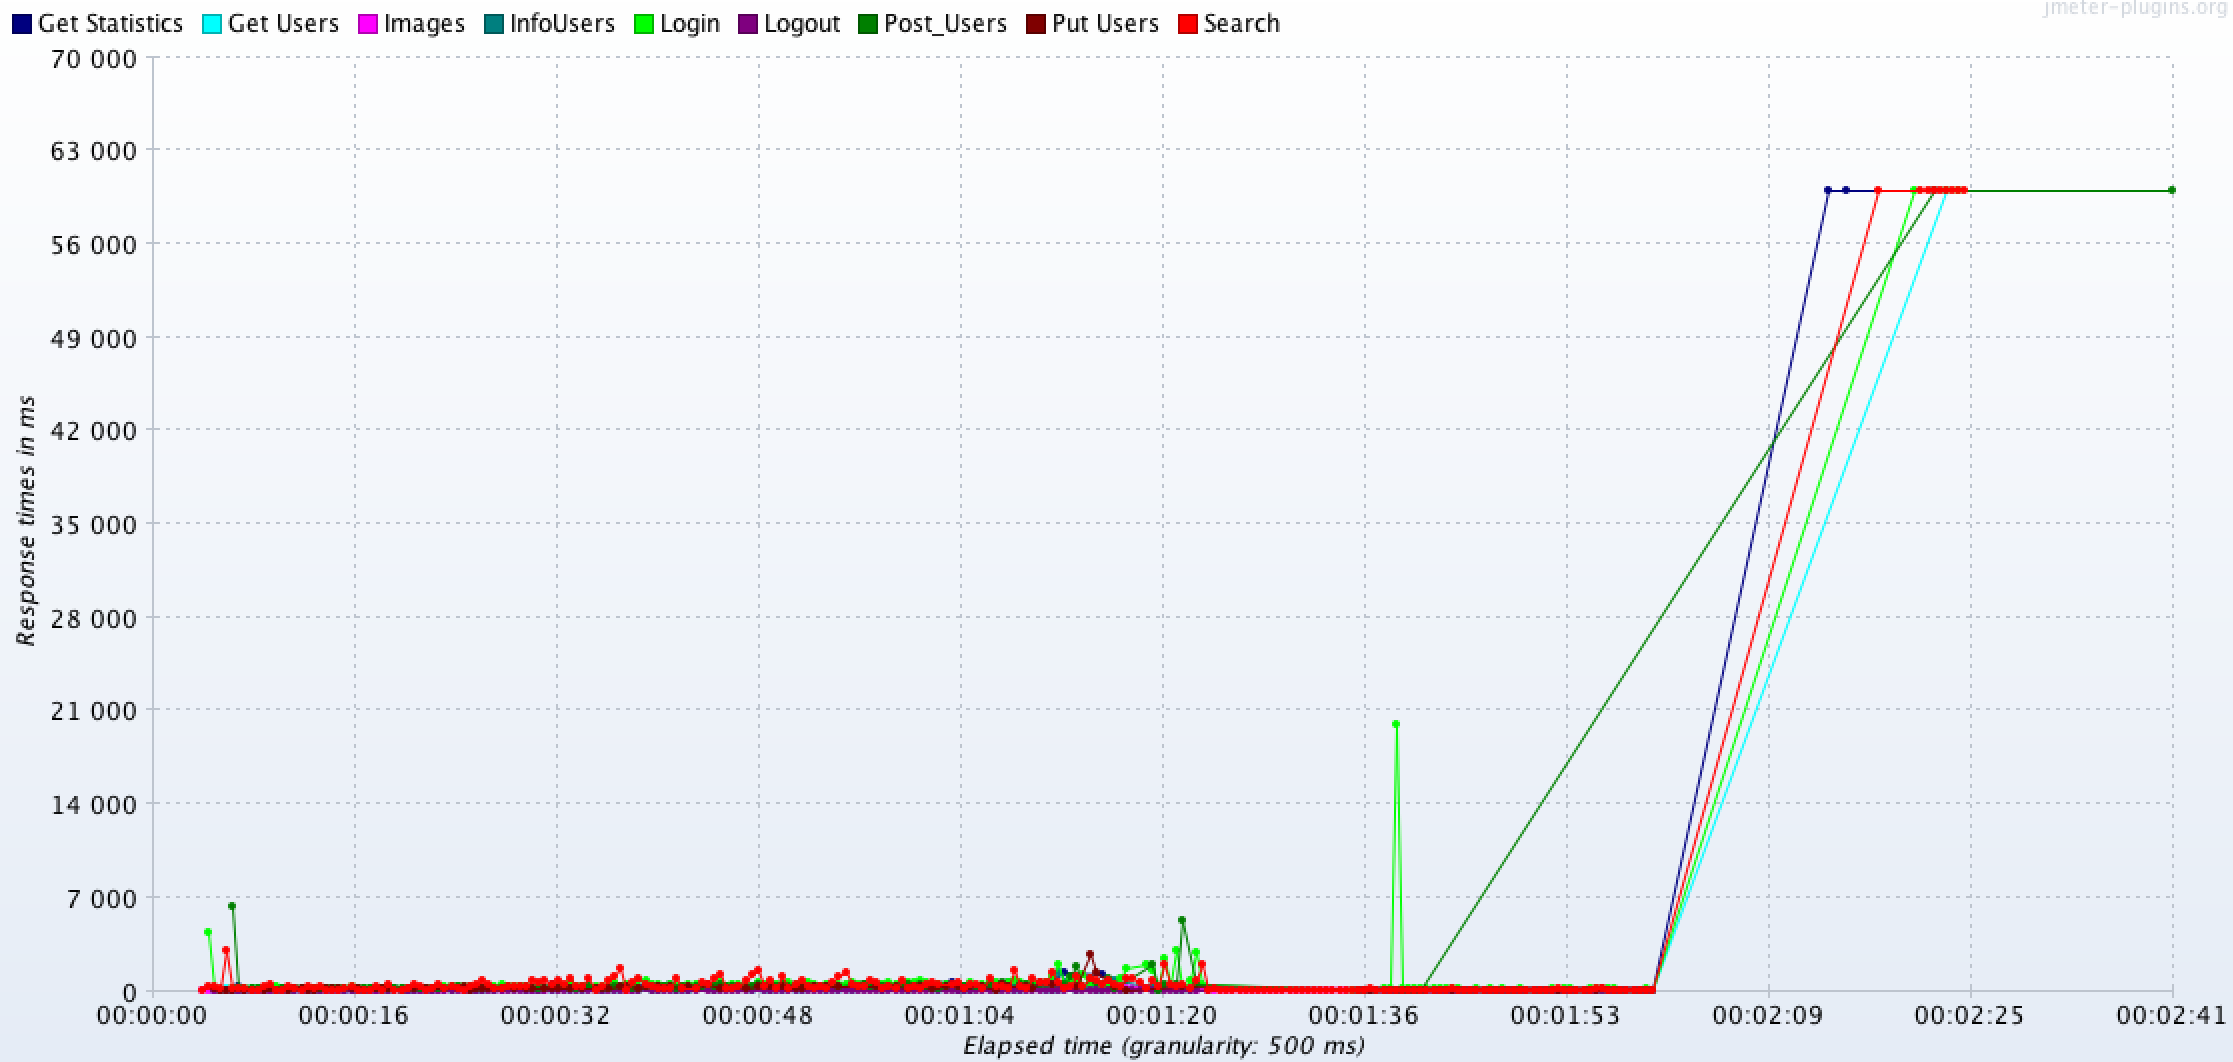
\includegraphics[width=1\textwidth]{images/Testes/3PC_RU_30R.png}
    \caption{Tempo de resposta aos pedidos efetuados ao longo do tempo, para o teste do tipo \textbf{2} com 30 utilizadores virtuais.}
    \label{fig:3PC_RU_30_response}
\end{figure}

\begin{table}[H]
\centering
\caption{Quantidade de sucessos e insucessos, bem com percentagem de insucesso, para o teste do tipo \textbf{2} com 30 utilizadores virtuais.}
\begin{tabular}{cccc}
\hline
\rowcolor[HTML]{EFEFEF} 
\textbf{Thread-Group}                  & \textbf{Sucesso} & \textbf{Insucesso} & \textbf{\% Insucesso} \\ \hline
\textbf{pesquisa c/ login}             & 1239             & 139                & 10,09\%               \\
\textbf{pesquisa s/ login}             & 3517             & 375                & 9,64\%                \\
\textbf{registo}                       & 893              & 99                 & 9,98\%                \\
\textbf{editar info pessoais}          & 680              & 1175               & 63,34\%               \\ \hline
\cellcolor[HTML]{EFEFEF}\textbf{Total} & 6329             & 1788               & 22,03\%               \\ \hline
\end{tabular}
\end{table}

Tendo os resultados deste teste em conta, percebe-se que 30 utilizadores virtuais para o teste do tipo 2, ainda é um valor demasiado elevado.

\vspace{0.5cm}
\noindent\textbf{Teste do tipo 2 com 20 utilizadores virtuais:}
%Teste RU 20
%throughput: 72,00s
%response: 233ms

Neste teste obteve-se um débito de 72 operações por segundo e um tempo de resposta médio de 233 milissegundos. Conforme esperado, estes valores ainda são aceitáveis e, para além disso, a taxa de insucesso também o passou a ser (7,35\%). 


\begin{figure}[H]
    \centering
    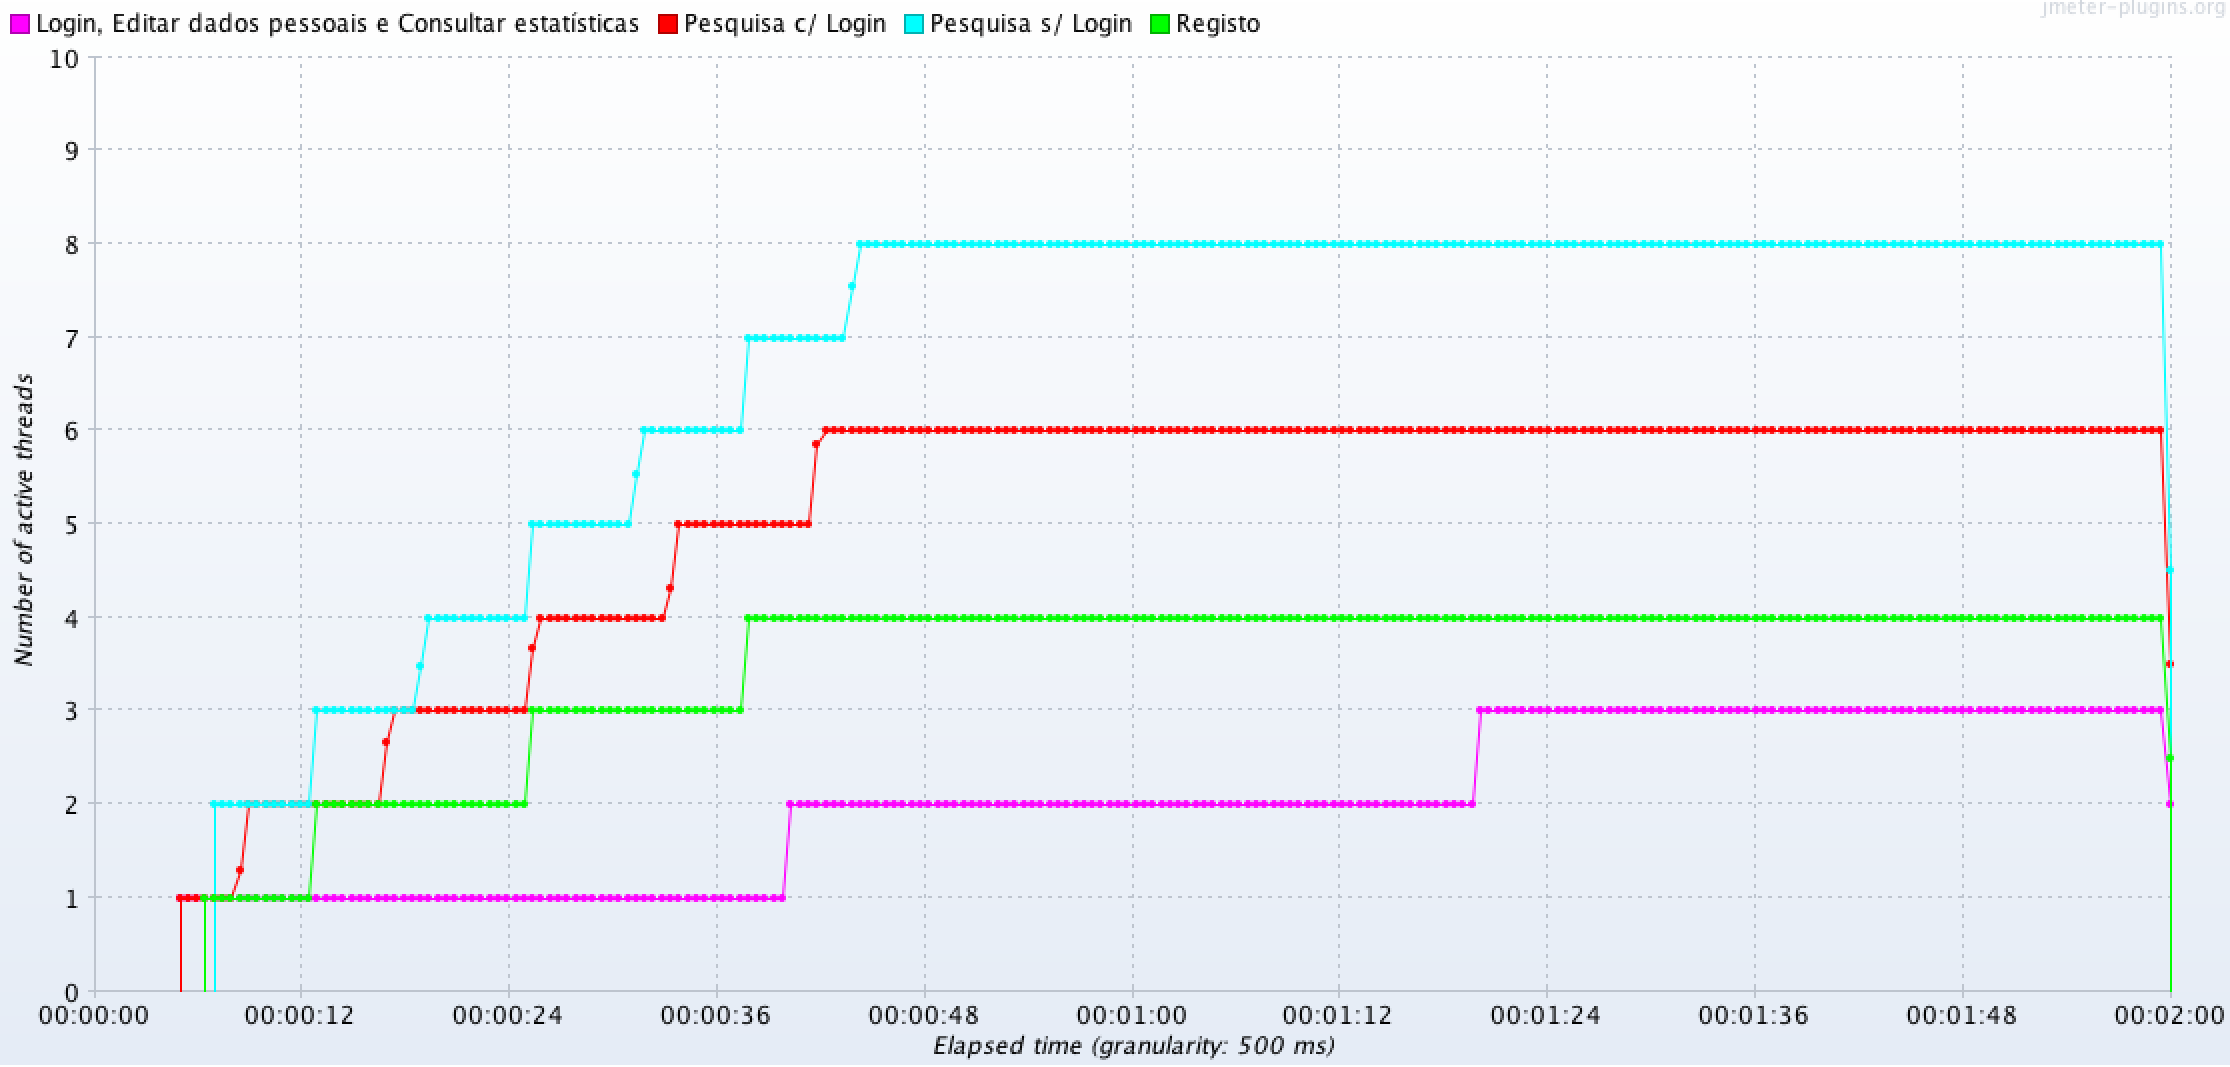
\includegraphics[width=1\textwidth]{images/Testes/3PC_RU_20T.png}
    \caption{Quantidade de \textit{threads} ativas ao longo do tempo, para o teste do tipo \textbf{2} com 20 utilizadores virtuais.}
    \label{fig:3PC_RU_20_threads}
\end{figure}

\begin{figure}[H]
    \centering
    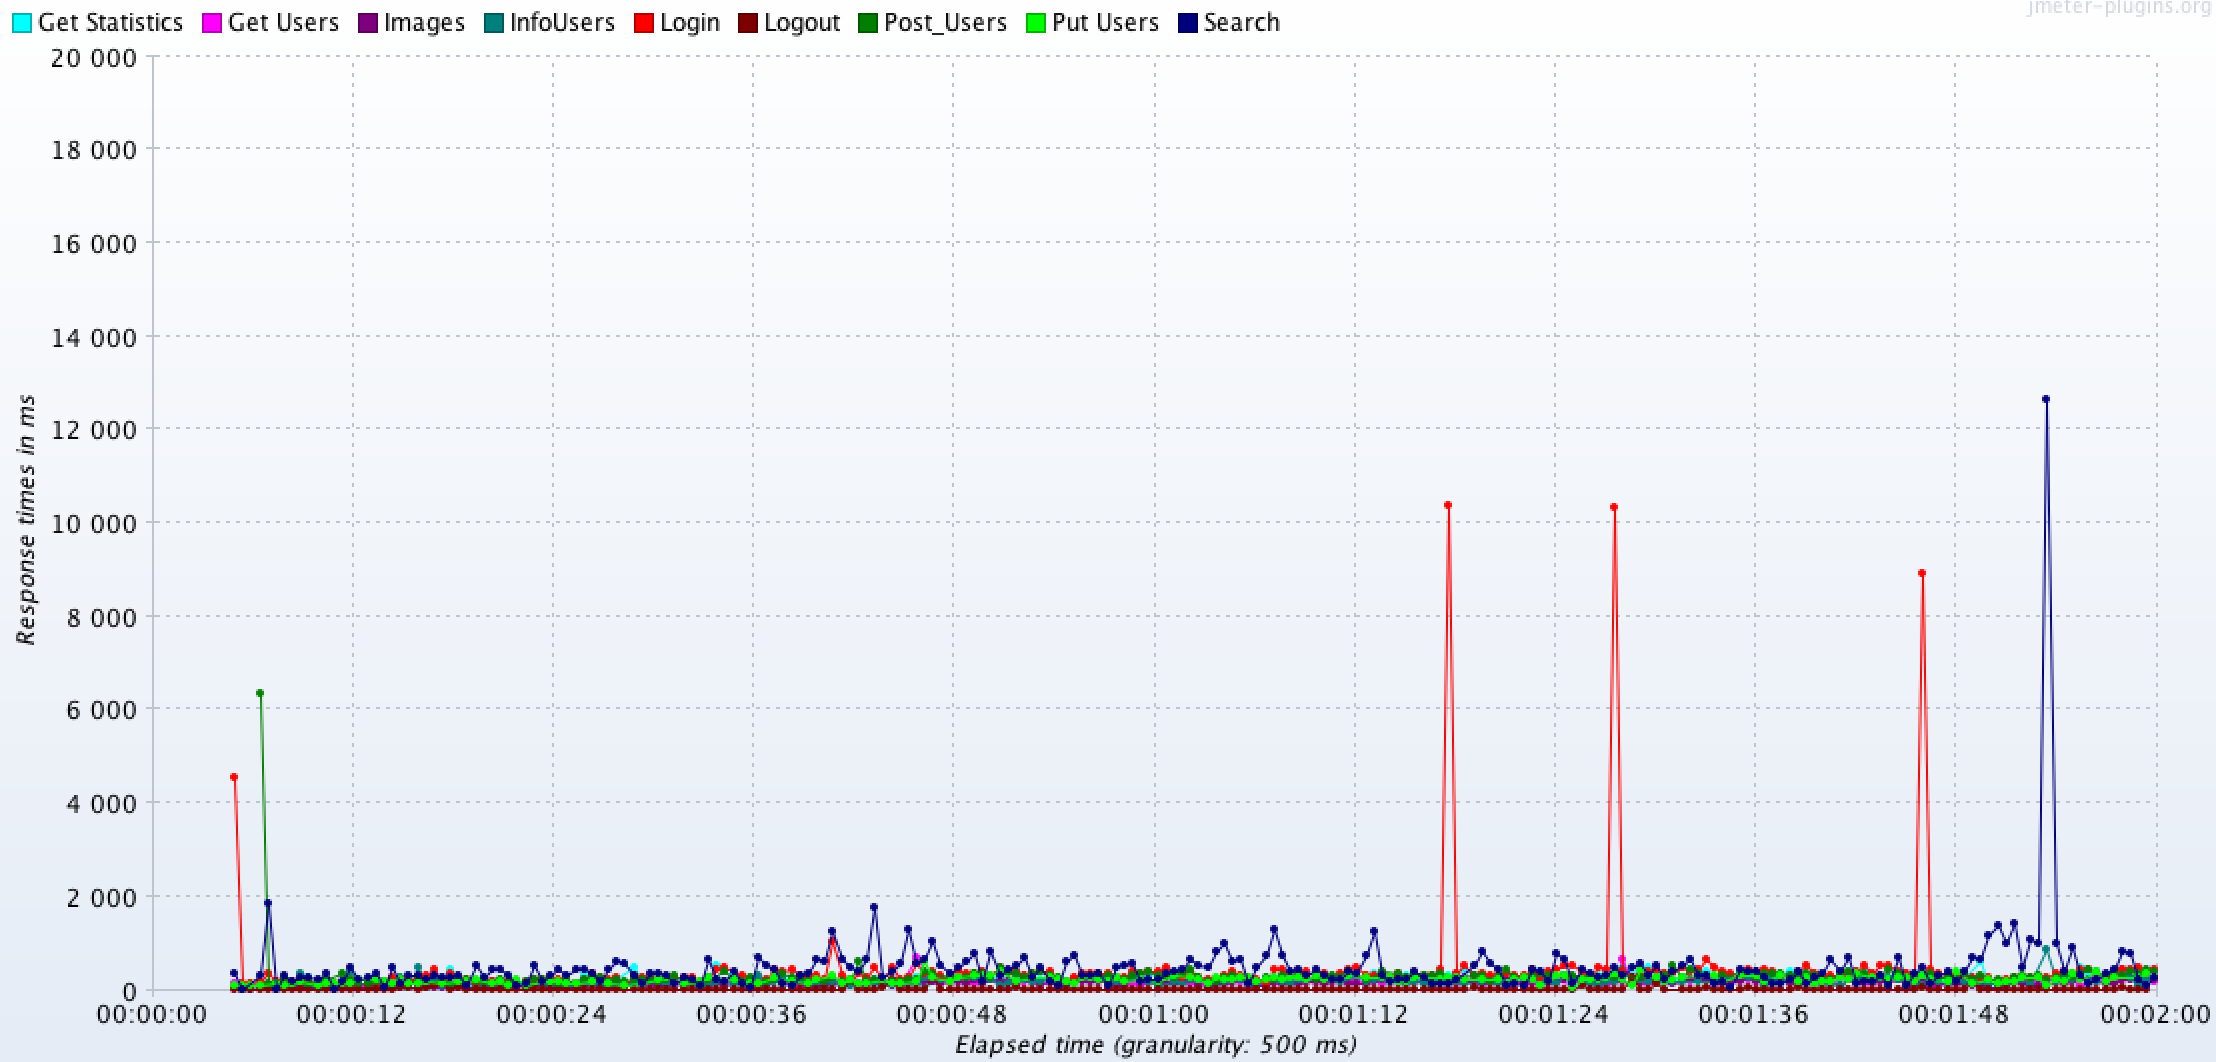
\includegraphics[width=1\textwidth]{images/Testes/3PC_RU_20R.png}
    \caption{Tempo de resposta aos pedidos efetuados ao longo do tempo, para o teste do tipo \textbf{2} com 20 utilizadores virtuais.}
    \label{fig:3PC_RU_20_response}
\end{figure}

\begin{table}[H]
\centering
\caption{Quantidade de sucessos e insucessos, bem com percentagem de insucesso, para o teste do tipo \textbf{2} com 20 utilizadores virtuais.}
\begin{tabular}{cccc}
\hline
\rowcolor[HTML]{EFEFEF} 
\textbf{Thread-Group}                  & \textbf{Sucesso} & \textbf{Insucesso} & \textbf{\% Insucesso} \\ \hline
\textbf{pesquisa c/ login}             & 2246             & 212                & 8,62\%                \\
\textbf{pesquisa s/ login}             & 3344             & 344                & 9,33\%                \\
\textbf{registo}                       & 1281             & 44                 & 3,32\%                \\
\textbf{editar info pessoais}          & 1153             & 37                 & 3,11\%                \\ \hline
\cellcolor[HTML]{EFEFEF}\textbf{Total} & 8024             & 637                & 7,35\%                \\ \hline
\end{tabular}
\end{table}


\paragraph{Arquitetura com dois Servidores Aplicacionais}\label{sec:app2}

\vspace{0.5cm}
\noindent\textbf{Teste do tipo 1 com 100 utilizadores virtuais:}
%Teste 100
%Throughput: 10,43s 
%Average: 468ms

Neste teste obteve-se um débito de 10,43 operações por segundo e um tempo de resposta médio de 468 milissegundos. Para além disso, obteve-se uma quantidade de \textit{threads} ativas aceitáveis (geralmente igual a 1 \textit{thread}, após estabilizar), como se pode verificar através da figura \ref{fig:4PC_100_threads}. Adicionalmente, verificou-se que a taxa de insucesso na receção de resposta encontra-se na ordem dos 1,38\%.

\begin{figure}[H]
    \centering
    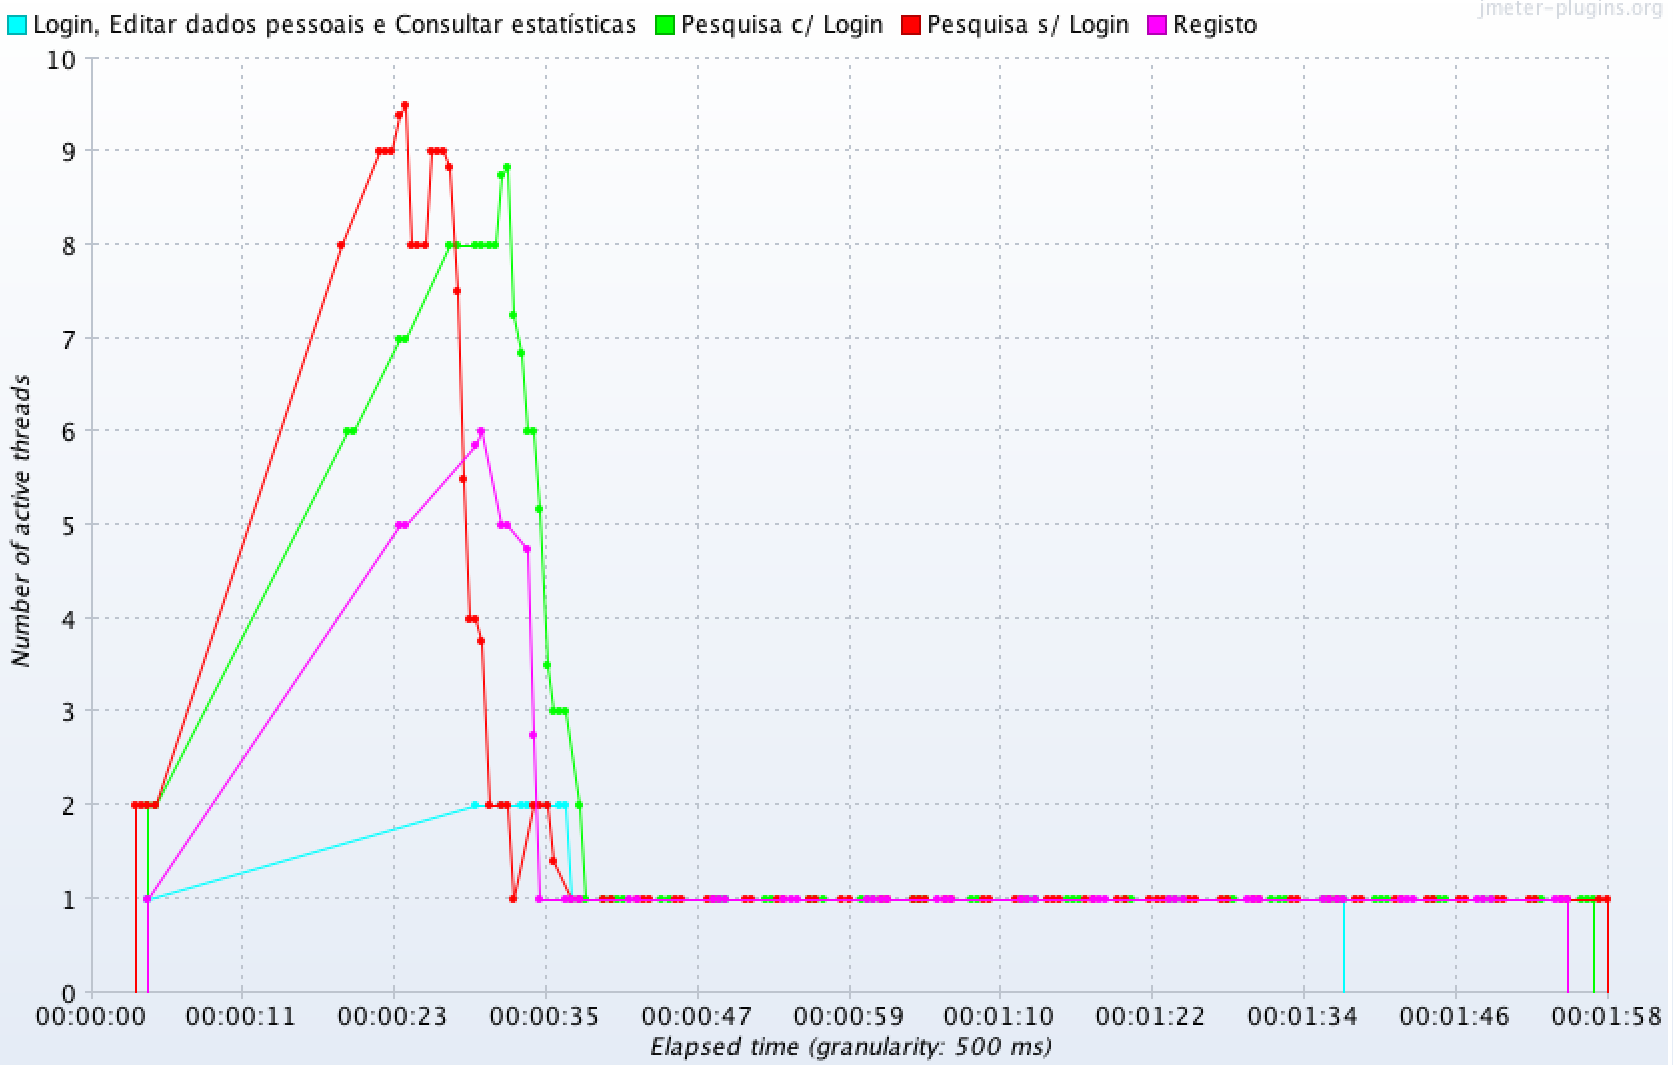
\includegraphics[width=1\textwidth]{images/Testes/4PC100T.png}
    \caption{Quantidade de \textit{threads} ativas ao longo do tempo, para o teste do tipo \textbf{1} com 100 utilizadores virtuais.}
    \label{fig:4PC_100_threads}
\end{figure}

\begin{figure}[H]
    \centering
    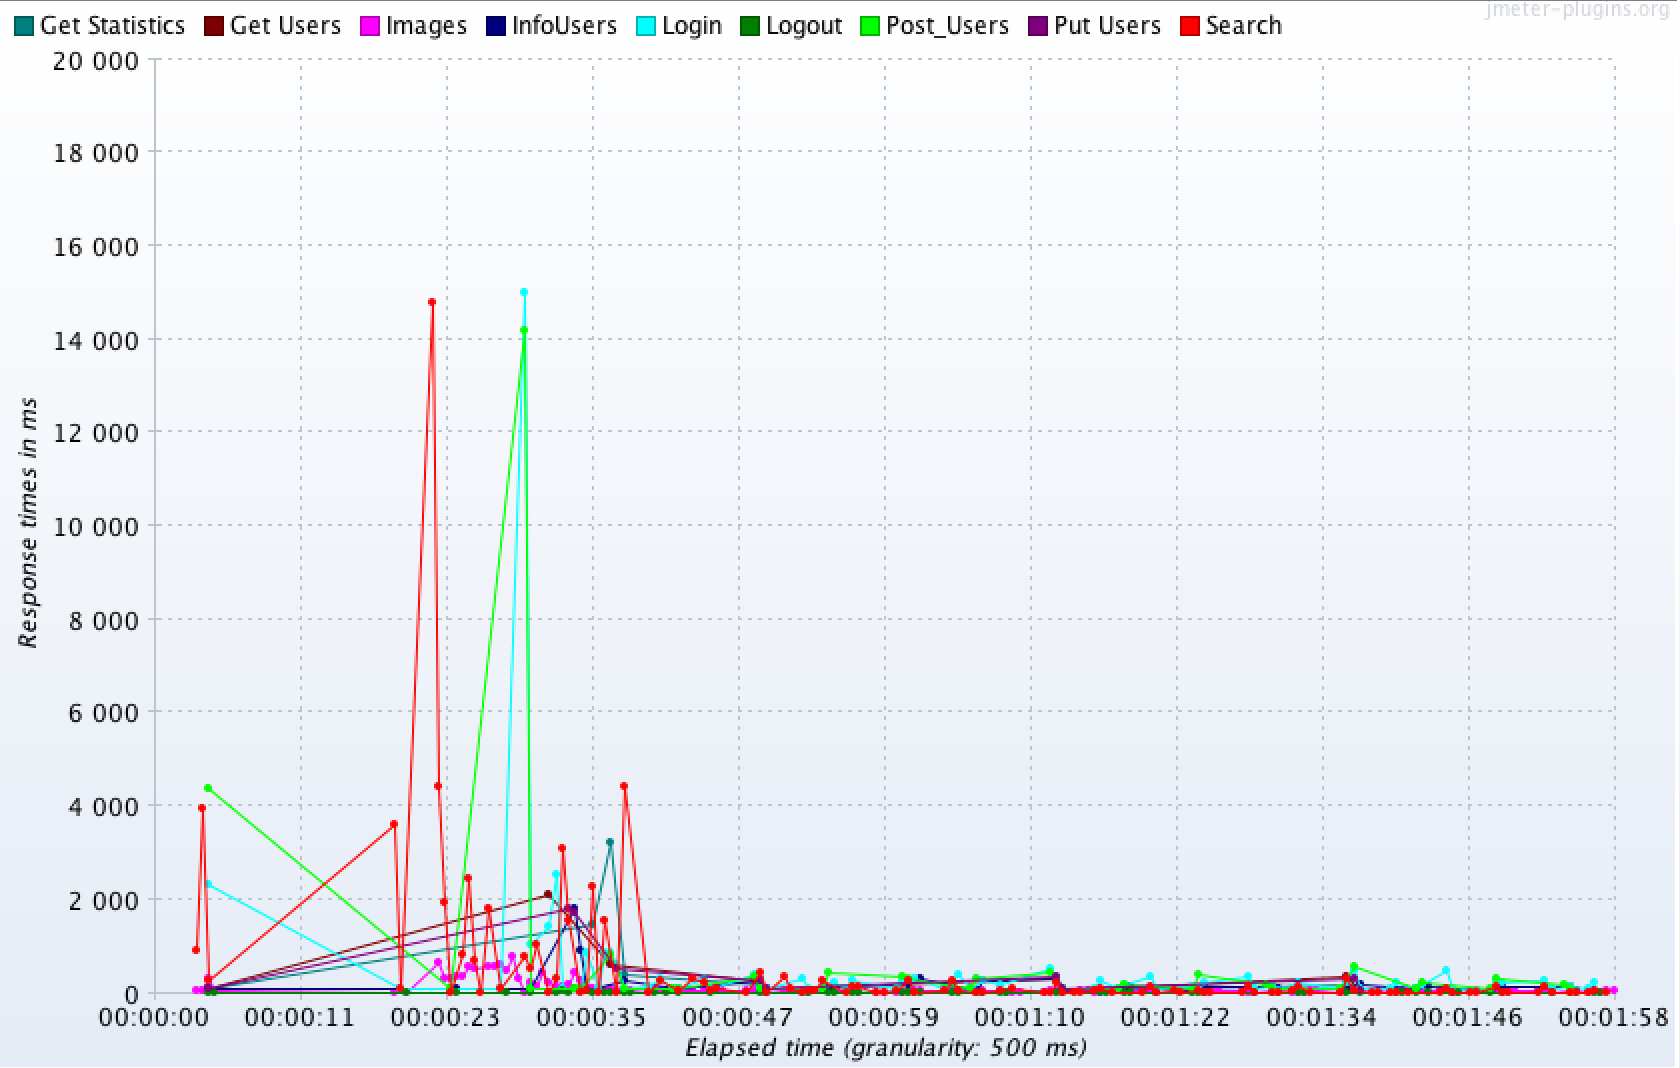
\includegraphics[width=1\textwidth]{images/Testes/4PC100R.png}
    \caption{Tempo de resposta aos pedidos efetuados ao longo do tempo, para o teste do tipo \textbf{1} com 100 utilizadores virtuais.}
    \label{fig:4PC_100_response}
\end{figure}

\begin{table}[H]
\centering
\caption{Quantidade de sucessos e insucessos, bem com percentagem de insucesso, para o teste do tipo \textbf{1} com 100 utilizadores virtuais.}
\begin{tabular}{cccc}
\hline
\rowcolor[HTML]{EFEFEF} 
\textbf{Thread-Group}                  & \textbf{Sucesso} & \textbf{Insucesso} & \textbf{\% Insucesso} \\ \hline
\textbf{pesquisa c/ login}             & 471              & 9                  & 1,88\%                \\
\textbf{pesquisa s/ login}             & 532              & 8                  & 1,48\%                \\
\textbf{registo}                       & 160              & 0                  & 0,00\%                \\
\textbf{editar info pessoais}          & 50               & 0                  & 0,00\%                \\ \hline
\cellcolor[HTML]{EFEFEF}\textbf{Total} & 1213             & 17                 & 1,38\%                \\ \hline
\end{tabular}
\end{table}

Com estes valores percebe-se que o servidor é capaz de dar resposta a mais pedidos (débito e tempo de resposta reduzidos, bem como reduzida percentagem de insucesso), pelo que se optou por aumentar a quantidade de utilizadores virtuais para este tipo de teste. 

\vspace{0.5cm}
\noindent\textbf{Teste do tipo 1 com 400 utilizadores virtuais:}
%Teste 400
%Troughput: 21,04 s  
%Average: 217 ms

Neste teste obteve-se um débito de 21,04 operações por segundo e um tempo de resposta médio de 217 milissegundos. Salienta-se que, conforme se pode perceber através do gráfico \ref{fig:4PC_400_response}, os pedidos iniciais ao servidor tiveram um tempo de resposta superior, relativamente ao teste anterior. Contudo, o servidor aplicacional foi capaz de estabilizar o tempo de resposta ao pedidos efetuados no mesmo período de tempo.

Relativamente à taxa de insucesso, este encontra-se na ordem dos 1,32\%.

\begin{figure}[H]
    \centering
    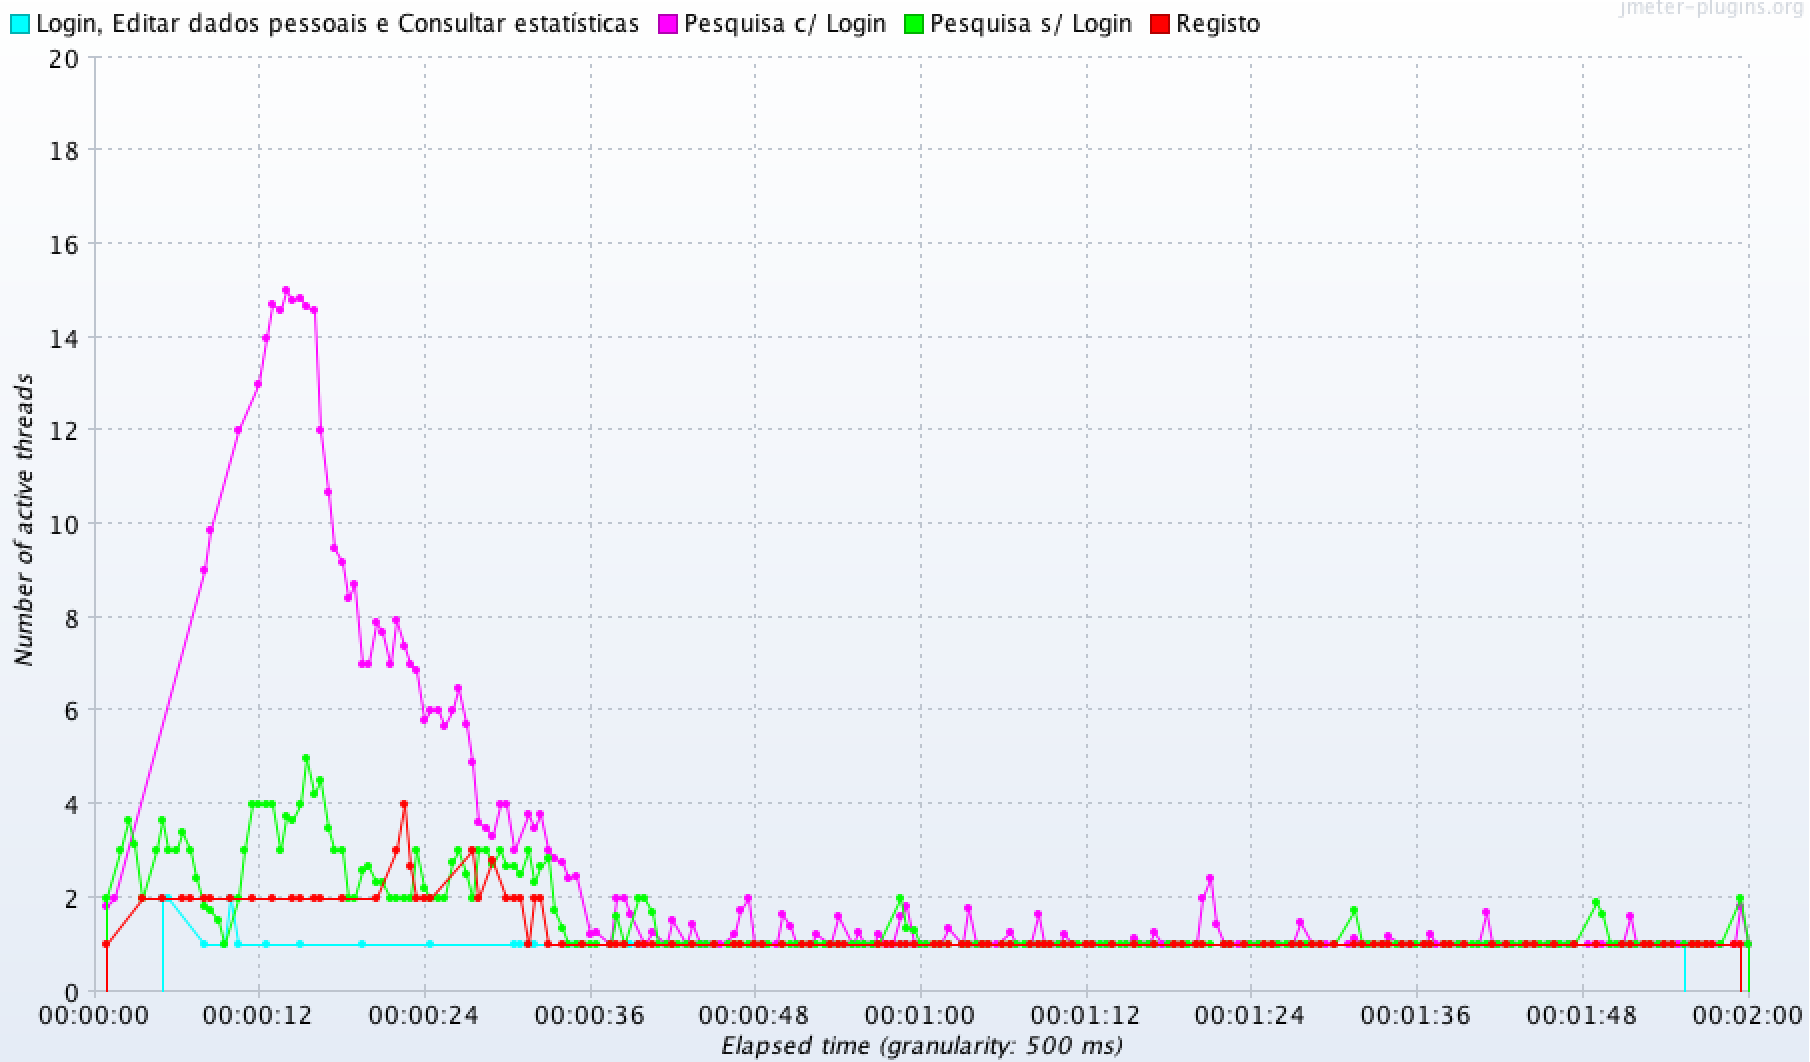
\includegraphics[width=1\textwidth]{images/Testes/4PCT400.png}
    \caption{Quantidade de \textit{threads} ativas ao longo do tempo, para o teste do tipo \textbf{1} com 400 utilizadores virtuais..}
    \label{fig:4PC_400_threads}
\end{figure}

\begin{figure}[H]
    \centering
    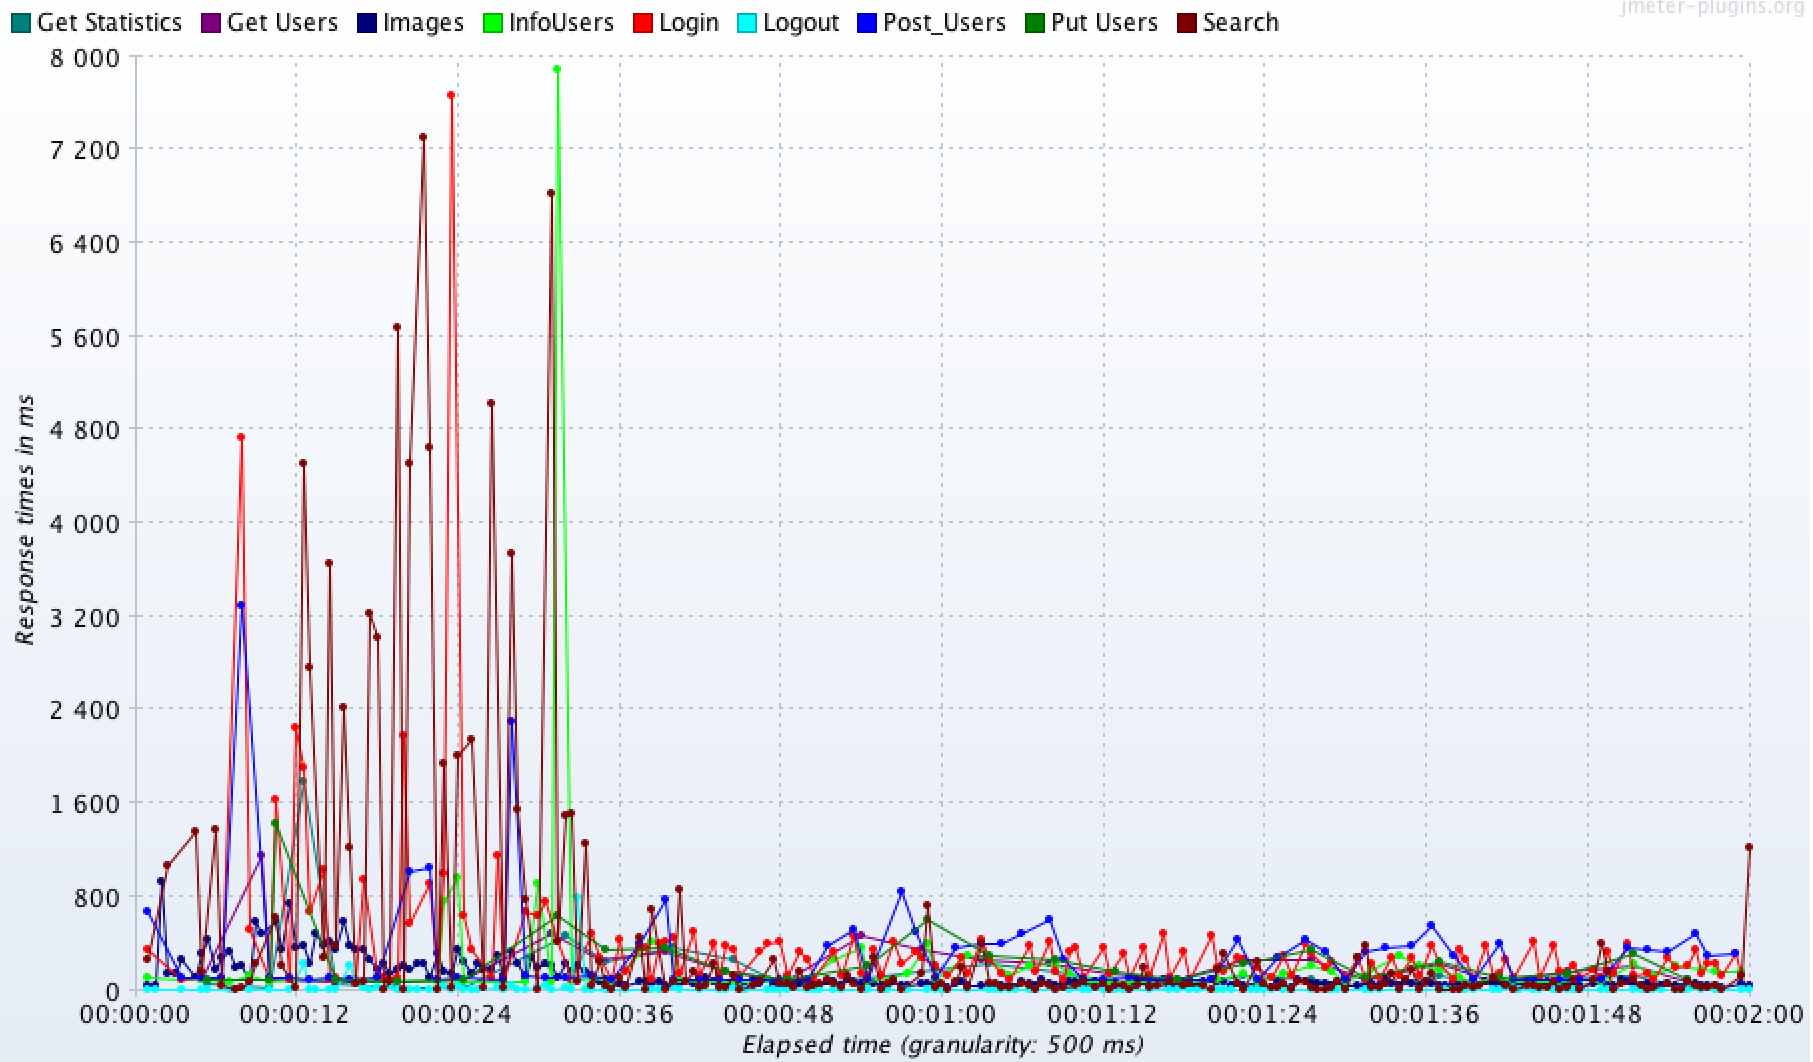
\includegraphics[width=1\textwidth]{images/Testes/4PCR400.png}
    \caption{Tempo de resposta aos pedidos efetuados ao longo do tempo, para o teste do tipo \textbf{1} com 400 utilizadores virtuais.}
    \label{fig:4PC_400_response}
\end{figure}

\begin{table}[H]
\centering
\caption{Quantidade de sucessos e insucessos, bem com percentagem de insucesso, para o teste do tipo \textbf{1} com 400 utilizadores virtuais.}
\begin{tabular}{cccc}
\hline
\rowcolor[HTML]{EFEFEF} 
\textbf{Thread-Group}                  & \textbf{Sucesso} & \textbf{Insucesso} & \textbf{\% Insucesso} \\ \hline
\textbf{pesquisa c/ login}             & 1181             & 19                 & 1,58\%                \\
\textbf{pesquisa s/ login}             & 889              & 11                 & 1,22\%                \\
\textbf{registo}                       & 297              & 3                  & 1,00\%                \\
\textbf{editar info pessoais}          & 248              & 2                  & 0,80\%                \\ \hline
\cellcolor[HTML]{EFEFEF}\textbf{Total} & 2615             & 35                 & 1,32\%                \\ \hline
\end{tabular}
\end{table}

Estes são resultados positivos, a partir dos quais se pode concluir que o servidor aplicacional é capaz de lidar com 400 utilizadores virtuais, num teste do tipo 1.

\vspace{0.5cm}
\noindent\textbf{Teste do tipo 2 com 100 utilizadores virtuais:}

%Teste RU 100
%throughput: 35,36s
%average: 2204ms

Agora, com o teste do tipo 2, obteve-se um débito de 35,36 operações por segundo e um tempo de resposta médio de 2,2 segundos.

Adicionalmente, verificou-se que a taxa de insucesso na receção de resposta se encontra na ordem dos 5,60\%.


\begin{figure}[H]
    \centering
    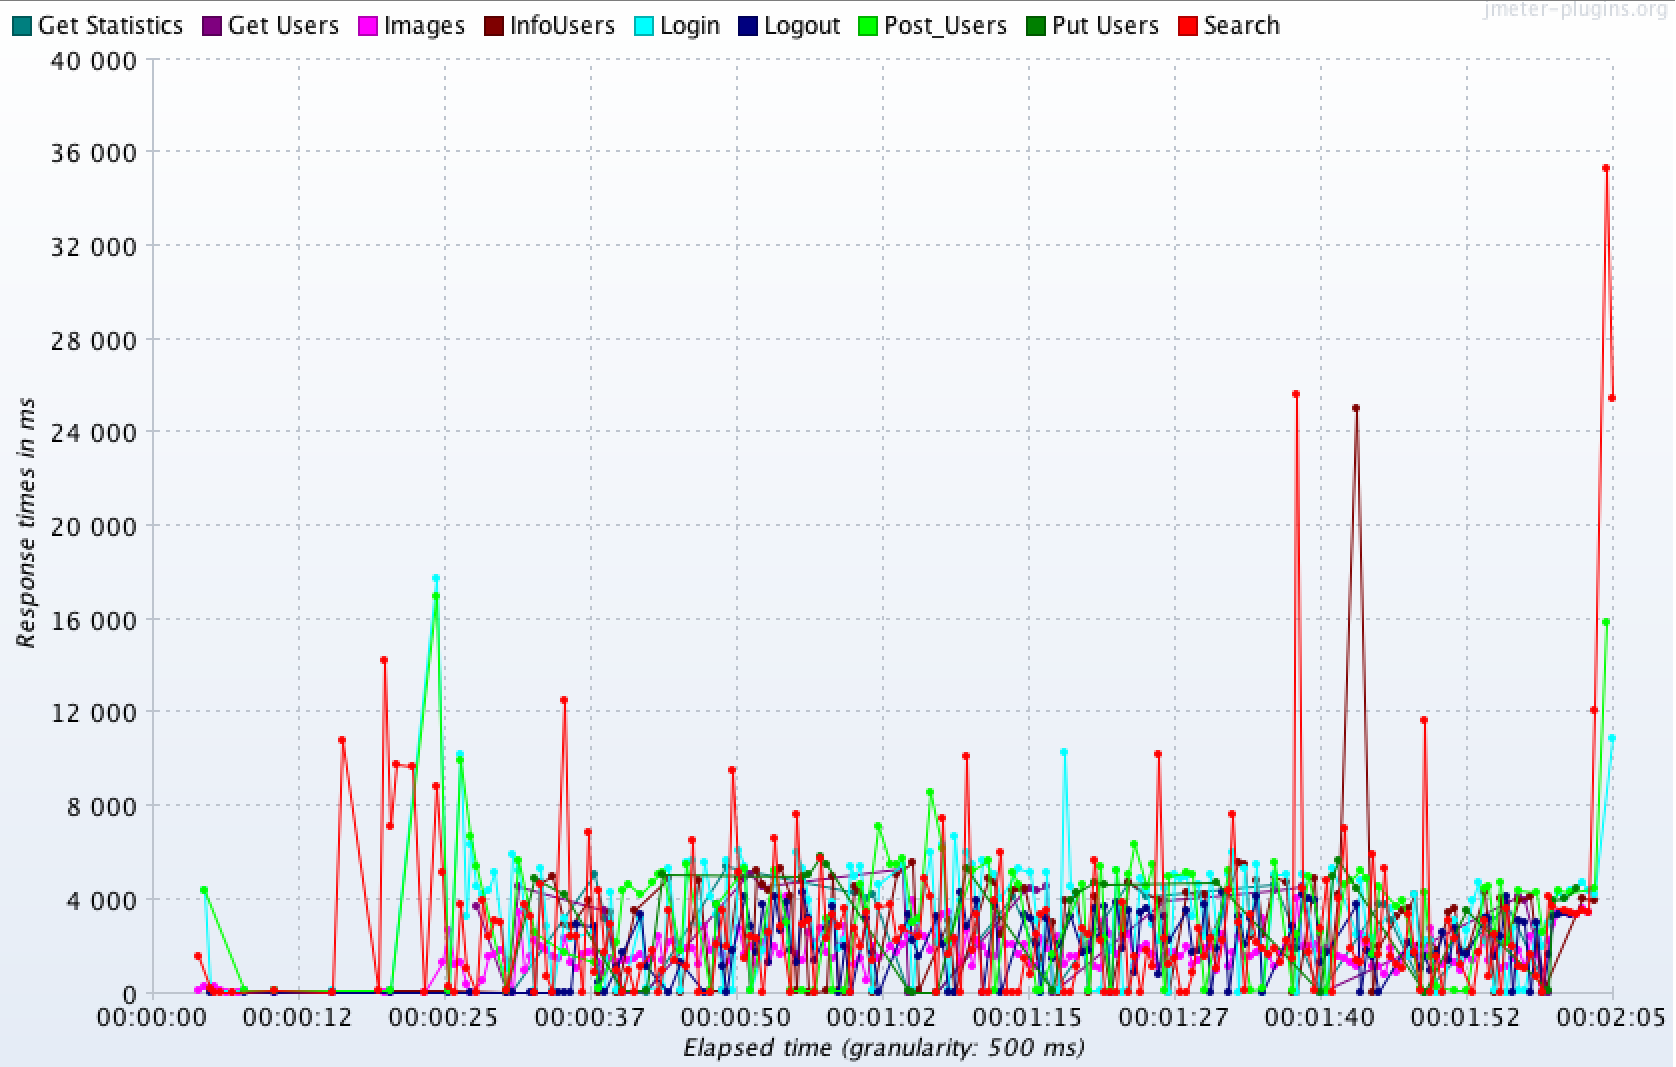
\includegraphics[width=1\textwidth]{images/Testes/4PC_RU100R.png}
    \caption{Quantidade de \textit{threads} ativas ao longo do tempo, para o teste do tipo \textbf{2} com 100 utilizadores virtuais.}
    \label{fig:4PC_RU_100_threads}
\end{figure}

\begin{figure}[H]
    \centering
    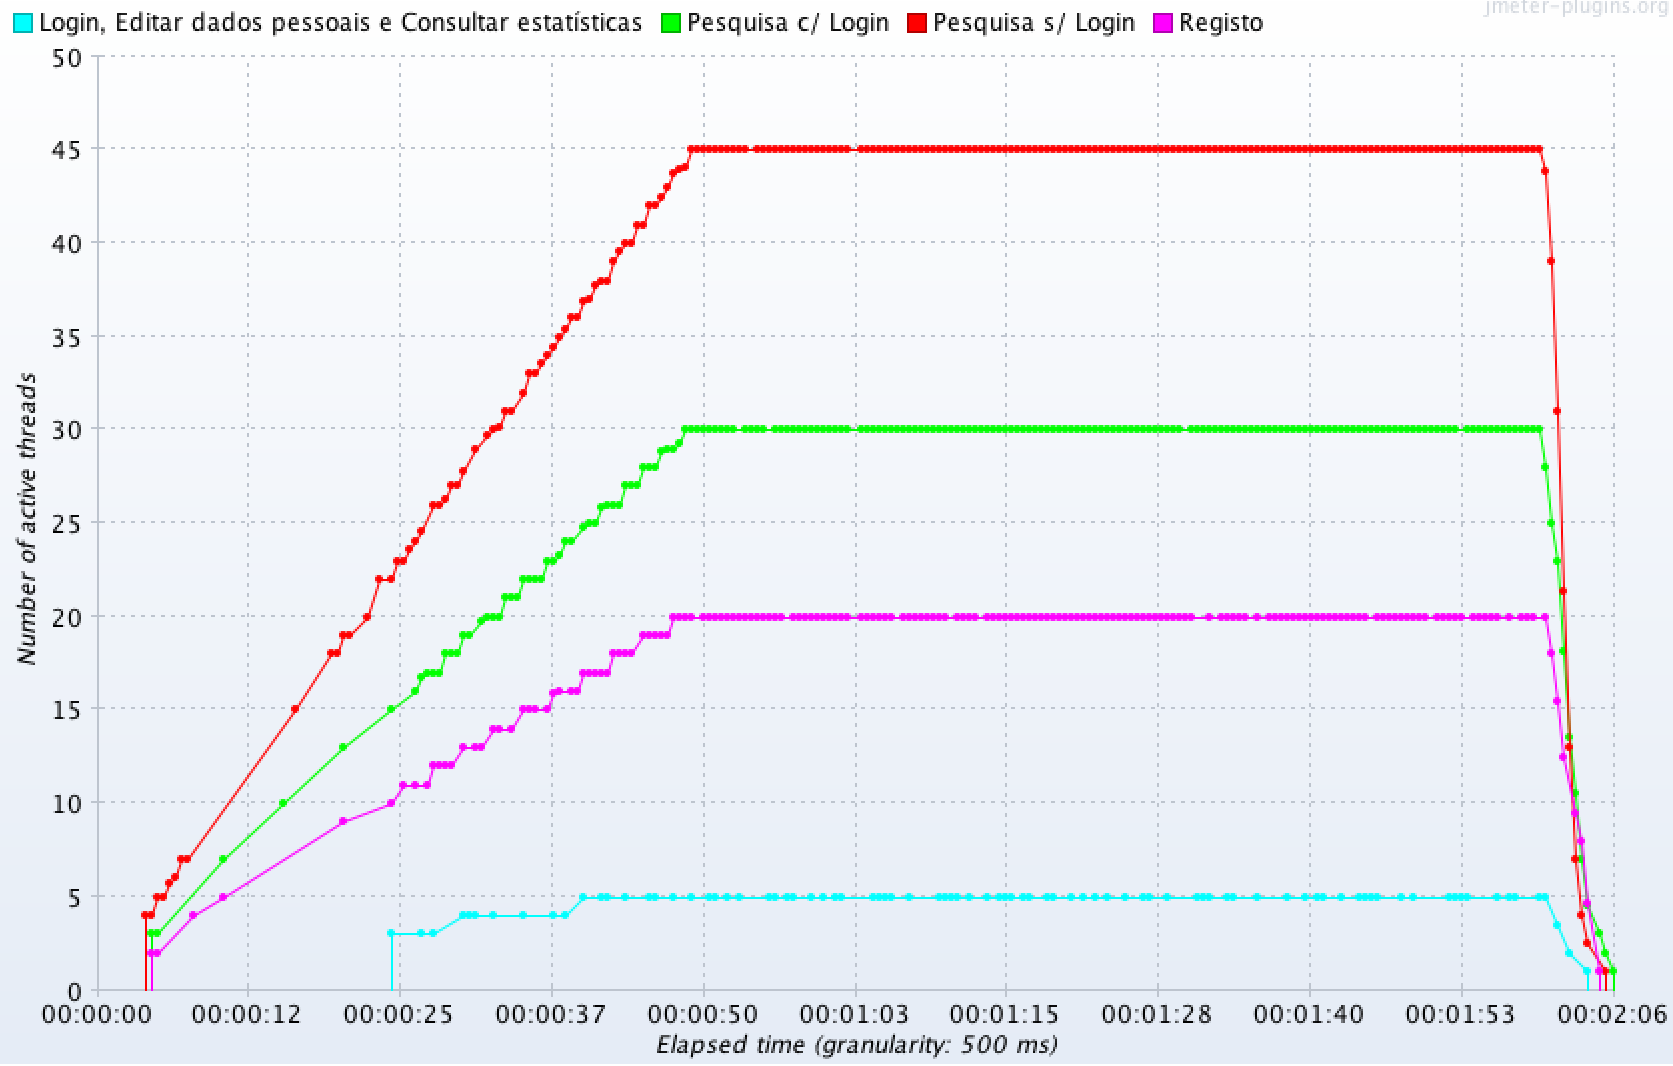
\includegraphics[width=1\textwidth]{images/Testes/4PC_RU100T.png}
    \caption{Tempo de resposta aos pedidos efetuados ao longo do tempo, para o teste do tipo \textbf{2} com 100 utilizadores virtuais.}
    \label{fig:4PC_RU_100_response}
\end{figure}

\begin{table}[H]
\centering
\caption{Quantidade de sucessos e insucessos, bem com percentagem de insucesso, para o teste do tipo \textbf{2} com 100 utilizadores virtuais.}
\begin{tabular}{cccc}
\hline
\rowcolor[HTML]{EFEFEF} 
\textbf{Thread-Group}                  & \textbf{Sucesso} & \textbf{Insucesso} & \textbf{\% Insucesso} \\ \hline
\textbf{pesquisa c/ login}             & 1064             & 84                 & 7,32\%                \\
\textbf{pesquisa s/ login}             & 2412             & 75                 & 3,02\%                \\
\textbf{registo}                       & 578              & 72                 & 11,08\%               \\
\textbf{editar info pessoais}          & 141              & 18                 & 11,32\%               \\ \hline
\cellcolor[HTML]{EFEFEF}\textbf{Total} & 4195             & 249                & 5,60\%                \\ \hline
\end{tabular}
\end{table}

Os tempos de resposta obtidos com este teste podem ser considerados ligeiramente negativos, uma vez que é frequente a ocorrência de tempos de resposta entre 2 e 8 segundos, tal como se pode verificar no gráfico apresentado na figura \ref{fig:4PC_RU_100_response}. Portanto, optou-se por reduzir a quantidade de utilizadores virtuais. 

\vspace{0.5cm}
\noindent\textbf{Teste do tipo 2 com 50 utilizadores virtuais:}

%Teste RU 50
%throughput: 36,81s
%average: 1078ms

Com este teste obteve-se um débito de 36,81 operações por segundo e um tempo de resposta médio de 1,08 segundos.

Adicionalmente, verificou-se que a taxa de insucesso na receção de resposta se encontra na ordem dos 3,17\%.

\begin{figure}[H]
    \centering
    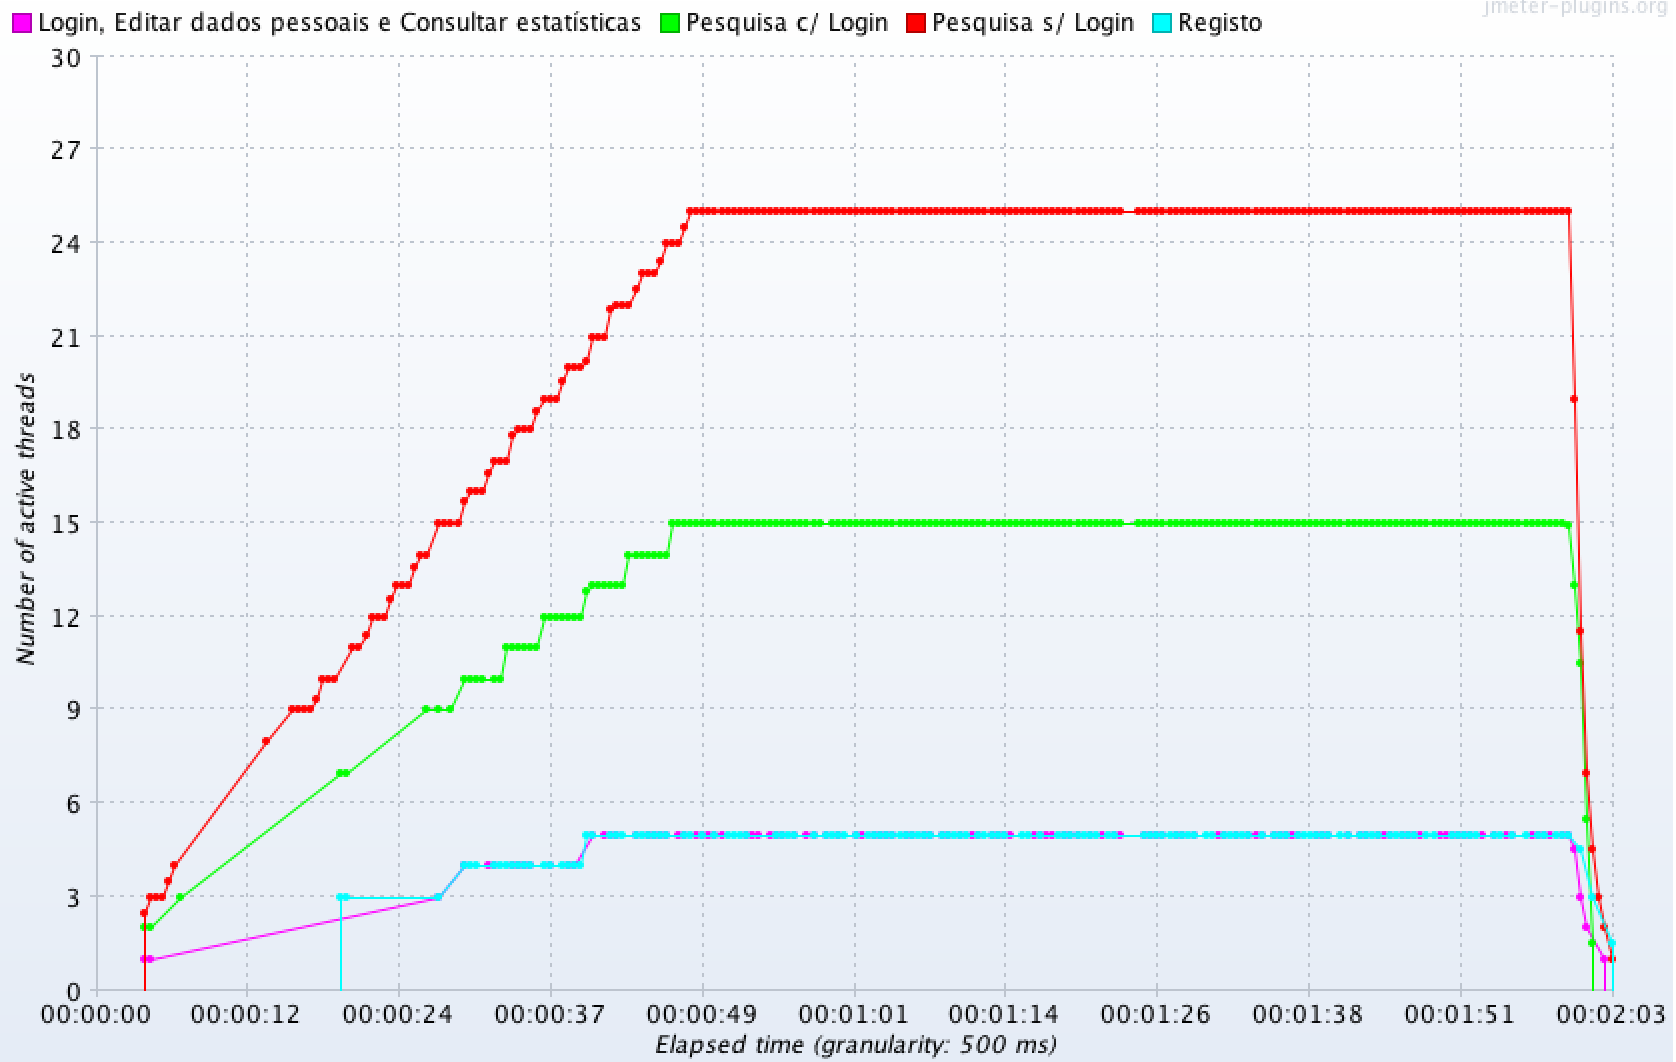
\includegraphics[width=1\textwidth]{images/Testes/4PC_RU50T.png}
    \caption{Quantidade de \textit{threads} ativas ao longo do tempo, para o teste do tipo \textbf{2} com 100 utilizadores virtuais.}
    \label{fig:4PC_RU_50_threads}
\end{figure}

\begin{figure}[H]
    \centering
    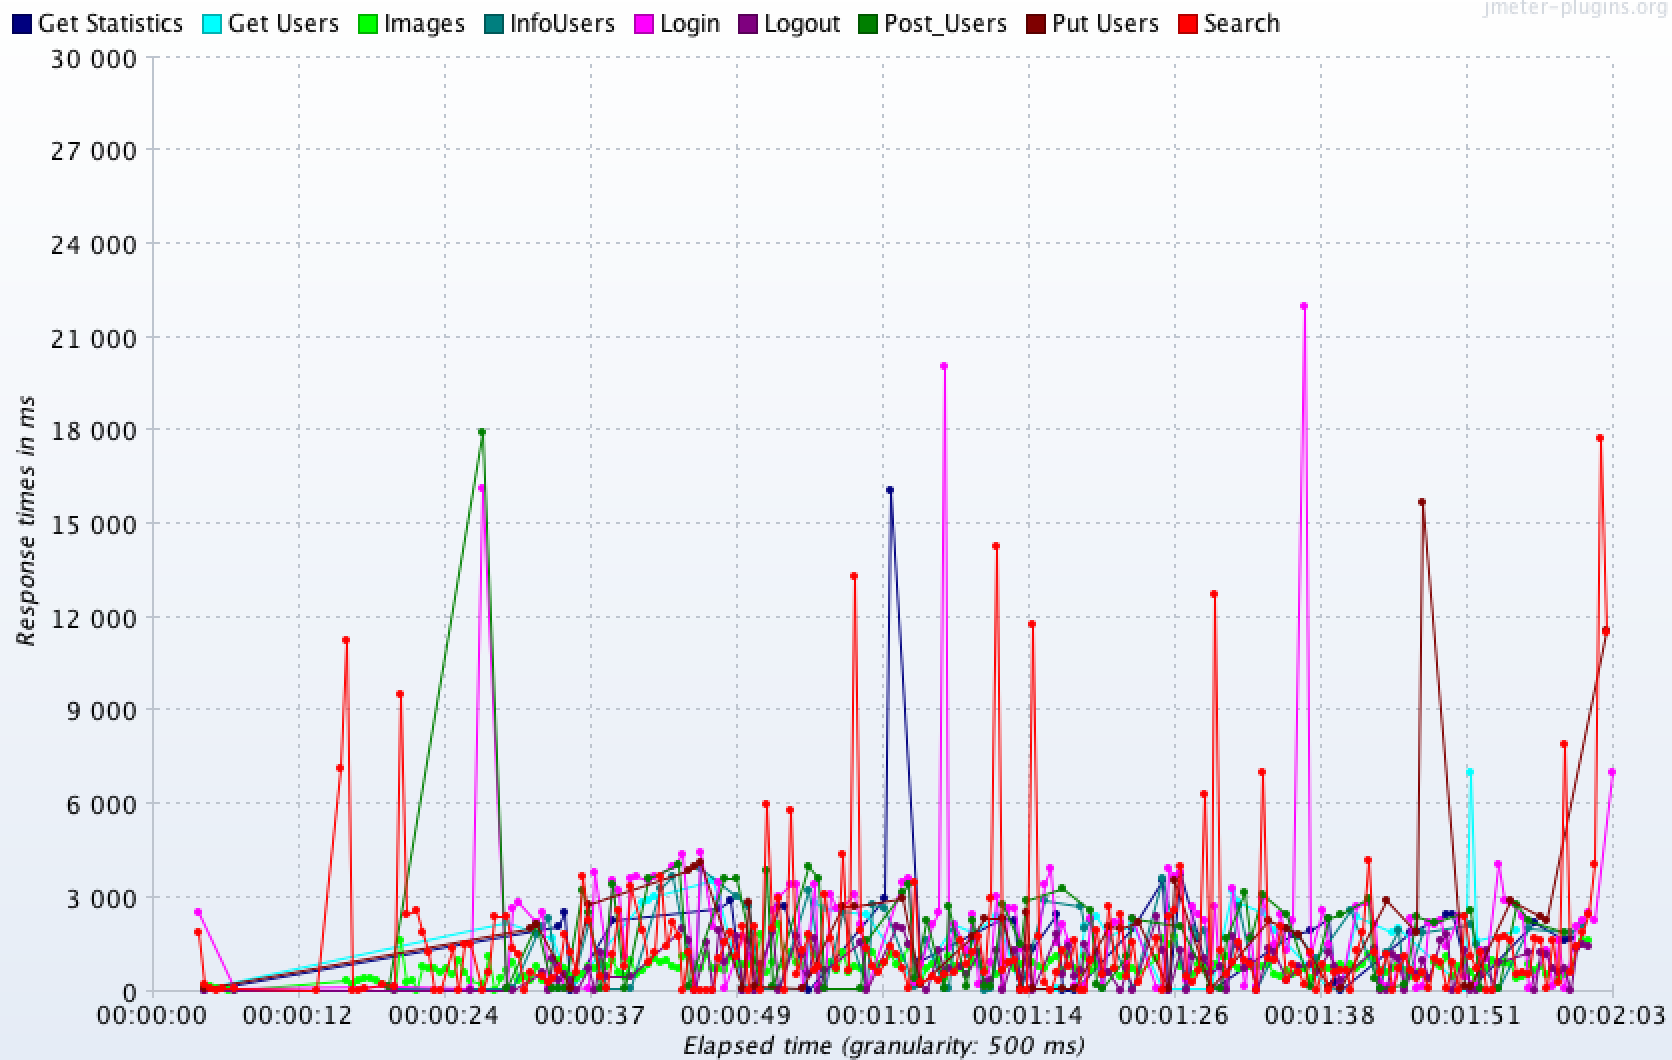
\includegraphics[width=1\textwidth]{images/Testes/4PC_RU50R.png}
    \caption{Tempo de resposta aos pedidos efetuados ao longo do tempo, para o teste do tipo \textbf{2} com 50 utilizadores virtuais.}
    \label{fig:4PC_RU_50_response}
\end{figure}

\begin{table}[H]
\centering
\caption{Quantidade de sucessos e insucessos, bem com percentagem de insucesso, para o teste do tipo \textbf{2} com 50 utilizadores virtuais.}
\begin{tabular}{cccc}
\hline
\rowcolor[HTML]{EFEFEF} 
\textbf{Thread-Group}                  & \textbf{Sucesso} & \textbf{Insucesso} & \textbf{\% Insucesso} \\ \hline
\textbf{pesquisa c/ login}             & 1028             & 44                 & 4,10\%                \\
\textbf{pesquisa s/ login}             & 2804             & 89                 & 3,08\%                \\
\textbf{registo}                       & 331              & 5                  & 1,49\%                \\
\textbf{editar info pessoais}          & 327              & 9                  & 2,68\%                \\ \hline
\cellcolor[HTML]{EFEFEF}\textbf{Total} & 4490             & 147                & 3,17\%                \\ \hline
\end{tabular}
\end{table}


Com este teste obtiveram-se valores de tempo de resposta um pouco melhores (com a maioria entre 0 e 4 segundos). Assim, considera-se que 50 utilizadores virtuais é o limite de carga para os servidores aplicacionais em testes do tipo 2.

\paragraph{Conclusões}

A partir dos resultados previamente apresentados, pode-se concluir que o servidor aplicacional tem como limite de carga 700 e 20 utilizadores virtuais para os testes de tipo 1 e 2, respetivamente. Para arquitetura com dois servidores aplicacionais, este limite de carga, manteve-se nos 400 e 50 utilizadores virtuais para os testes de tipo 1 e 2, respetivamente.

Salienta-se que para os testes com a arquitetura de dois servidores aplicacionais, um destes servidores estava a correr o \texttt{docker} da aplicação numa máquina virtual, com características muito inferiores às desejáveis. Desta forma, os resultados obtidos não são tão positivos conforme o esperado, em resultado da inclusão de uma nova máquina na arquitetura.

Por fim, é ainda de se referir que a quantidade de dados transferidos nas respostas aos pedidos HTTP é relativamente elevado, devido à transferência de imagens, conforme se pode verificar através dos dados apresentados na figura \ref{tab:bytes}.

\begin{table}[H]
\centering
\caption{Quantidade de dados transferidos nas respostas aos pedidos HTTP.}
\label{tab:bytes}
\begin{tabular}{ccccc}
\hline
\rowcolor[HTML]{EFEFEF} 
\textbf{\begin{tabular}[c]{@{}c@{}}Nº de Servidores\\ Aplicacionais\end{tabular}} & \textbf{\begin{tabular}[c]{@{}c@{}}Tipo de\\ Teste\end{tabular}} & \textit{\textbf{\begin{tabular}[c]{@{}c@{}}Number of\\ Threads\end{tabular}}} & \textbf{\begin{tabular}[c]{@{}c@{}}Quantidade de dados\\ transferidos (MB)\end{tabular}} \\ \hline
                                                                                  & 1                                                                & 700                                                                           & 820                                                                                      \\
\multirow{-2}{*}{1}                                                               & 2                                                                & 20                                                                            & 780                                                                                      \\ \hline
                                                                                  & 1                                                                & 400                                                                           & 510                                                                            \\
\multirow{-2}{*}{2}                                                               & 2                                                                & 50                                                                            & 260                                                                                      \\ \hline
\end{tabular}
\end{table}
